\documentclass[twoside, 11pt]{article}
\usepackage{../estilo-apuntes}
%\usepackage{amsmath,amssymb}
%\usepackage[utf8]{inputenc}
%\usepackage[spanish]{babel}
%\usepackage{caption}
%\usepackage[]{graphicx}
%\usepackage{enumerate}
%\usepackage{amsthm}
%\usepackage{tikz-cd}
%\usetikzlibrary{babel}
%\usepackage{pgf,tikz}
%\usepackage{mathrsfs}
%\usepackage{bm}  
%\usetikzlibrary{arrows}
%\usetikzlibrary{cd}
%\usepackage[spanish]{babel}
%\usepackage{fancyhdr}
%\usepackage{titlesec}
%\usepackage{floatrow}
%\usepackage{makeidx}
%\usepackage[tocflat]{tocstyle}
%\usetocstyle{standard}
%\usepackage{subfiles}
%\usepackage{color}  
%\usepackage{hyperref}
%\hypersetup{colorlinks=true,citecolor=red, linkcolor=blue}
%\usepackage{eurosym}
%%\usepackage{ntheorem}
%
%
%\renewcommand{\baselinestretch}{1,4}
%\setlength{\oddsidemargin}{0.25in}
%\setlength{\evensidemargin}{0.25in}
%\setlength{\textwidth}{6in}
%\setlength{\topmargin}{0.1in}
%\setlength{\headheight}{0.1in}
%\setlength{\headsep}{0.1in}
%\setlength{\textheight}{8in}
%\setlength{\footskip}{0.75in}
%
%\theoremstyle{definition}
%
%\newtheorem{teorema}{Teorema}[section]
%\newtheorem{defi}[teorema]{Definición}
%\newtheorem{coro}[teorema]{Corolario}
%\newtheorem{lemma}[teorema]{Lema}
%\newtheorem{ej}[teorema]{Ejemplo}
%\newtheorem{ejs}[teorema]{Ejemplos}
%\newtheorem{observacion}[teorema]{Observación}
%\newtheorem{observaciones}[teorema]{Observaciones}
%\newtheorem{prop}[teorema]{Proposición}
%\newtheorem{propi}[teorema]{Propiedades}
%\newtheorem{nota}[teorema]{Nota}
%\newtheorem{notas}[teorema]{Notas}
%\newtheorem*{dem}{Demostración}
%\newtheorem{ejer}[teorema]{Ejercicio}
%\newtheorem{problem}[teorema]{Problema}
%\newtheorem{concl}[teorema]{Conclusión}
%
%\providecommand{\abs}[1]{\lvert#1\rvert}
%\providecommand{\sen}[1]{sen #1}
%\providecommand{\norm}[1]{\lVert#1\rVert}
%\providecommand{\ninf}[1]{\norm{#1}_\infty}
%\providecommand{\numn}[1]{\norm{#1}_1}
%\providecommand{\gabs}[1]{\left|{#1}\right|}
%\newcommand{\bor}[1]{\mathcal{B}(#1)}
%\newcommand{\R}{\mathbb{R}}
%\newcommand{\Z}{\mathbb{Z}}
%\newcommand{\N}{\mathbb{N}}
%\newcommand{\Q}{\mathbb{Q}}
%\newcommand{\C}{\mathbb{C}}
%\newcommand{\Pro}{\mathbb{P}}
%\newcommand{\Tau}{\mathcal{T}}
%\newcommand{\verteq}{\rotatebox{90}{$\,=$}}
%\newcommand{\vertequiv}{\rotatebox{110}{$\,\equiv$}}
%\providecommand{\lrg}{\longrightarrow}
%\providecommand{\func}[2]{\colon{#1}\longrightarrow{#2}}
%\newcommand*{\QED}{\hfill\ensuremath{\blacksquare}}
%\newcommand*\circled[1]{\tikz[baseline=(char.base)]{
%            \node[shape=circle,draw,inner sep=1.5pt] (char) {#1};}}
%\newcommand*{\longhookarrow}{\ensuremath{\lhook\joinrel\relbar\joinrel\rightarrow}}


\begin{document}
%\title{Topología de Superficies}
%\author{Antonio Rafael Quintero Toscano\\ Javier Aguilar Martín}
%\date{Curso 2016/2017}
%\maketitle

\author{Javier Aguilar Martín }
\date{\today}
\title{Teoría Geométrica de Grupos}

\maketitle


\begin{abstract}
Estos apuntes están basados en las clases de Yago Antolín en la Escuela JAE de 2018. Sus notas originales pueden ser encontradas en el siguiente enlace: \url{https://sites.google.com/site/yagoanpi/curso-escuela-jae}
\end{abstract}


	\vfill
	Esta obra está licenciada bajo la Licencia Creative Commons Atribución 3.0 España. Para ver una copia de esta licencia, visite \url{http://creativecommons.org/licenses/by/3.0/es/} o envíe una carta a Creative Commons, PO Box 1866, Mountain View, CA 94042, USA.


\newpage
\tableofcontents

\newpage

\section{Grupos finitamente generados como espacios métricos}
\subsection{Grafos de Cayley}
\begin{teorema}[Cayley]
Todo subgrupo es isomorfo a un subgrupo de un grupo simétrico.
\end{teorema}
\begin{dem}
Dado un grupo $G$ definimos $\sigma:G\to Biy(G)=Sym_{|G|}$ como $x\mapsto \sigma_x:G\to G$, siendo $\sigma_x(g)=gx^{-1}$. Tenemos que $\sigma$ es un homomorfismo pues
$$
\sigma_{xy}(g)=g(xy)^{-1}=gy^{-1}x^{-1}=(gy^{-1})x^{-1})=\sigma_y(g)x^{-1}=\sigma_x(\sigma_y(g)).
$$
Además es inyectiva pues 
$$
\sigma_x(g)=g\Leftrightarrow gx^{-1}=g\Leftrightarrow x^{-1}=1_G\Leftrightarrow x=1_G.
$$
\QED
\end{dem}

\begin{ej}
Vamos a cómo se interpreta la demostración anterior en un ejemplo concreto. Sea $G=(\Z/3\Z)^3$ y sean $x=(1,0,0)$, $y=(0,1,0)$, $z=(0,0,1)$. Tenemos 
\[
\sigma_x\equiv (000,\ 100)(010,\ 110)(001,\ 101)(011,\ 111)
\]
expresada como producto de ciclos en los que los grupos de tres números se corresponden a su vez a ciclos. Análogamente se definirían $\sigma_y$ y $\sigma_z$. Podemos interpretar geométricamente estas aplicaciones como la acción que intercambia los vértices de un cubo como en la figura siguiente.

\definecolor{qqffqq}{rgb}{0.,1.,0.}
\definecolor{ffqqqq}{rgb}{1.,0.,0.}
\definecolor{qqqqff}{rgb}{0.,0.,1.}
\begin{tikzpicture}[line cap=round,line join=round,>=triangle 45,x=1.0cm,y=1.0cm, scale=0.9]
\clip(-3.3233333333333337,-1) rectangle (15.843333333333337,6);
\draw [->,line width=2.pt,color=qqqqff] (-0.23333333333333334,0.) -- (-0.22,3.993333333333332);
\draw [->,line width=2.pt,color=qqqqff] (0.22,3.993333333333332) -- (0.24666666666666667,0.);
\draw [->,line width=2.pt,color=qqqqff] (1.7533333333333334,0.9933333333333342) -- (1.7666666666666668,4.966666666666665);
\draw [->,line width=2.pt,color=qqqqff] (2.2333333333333334,4.993333333333331) -- (2.22,1.0066666666666677);
\draw [->,line width=2.pt,color=qqqqff] (5.78,0.98) -- (5.78,4.993333333333332);
\draw [->,line width=2.pt,color=qqqqff] (6.233333333333333,4.993333333333331) -- (6.22,0.953333333333334);
\draw [->,line width=2.pt,color=qqqqff] (3.78,0.) -- (3.7933333333333334,3.98);
\draw [->,line width=2.pt,color=qqqqff] (4.206666666666667,3.9666666666666655) -- (4.22,0.);
\draw [->,line width=2.pt,color=ffqqqq] (0.,0.23333333333333467) -- (4.006666666666667,0.23333333333333467);
\draw [->,line width=2.pt,color=ffqqqq] (3.9933333333333336,-0.22) -- (0.,-0.23333333333333164);
\draw [->,line width=2.pt,color=ffqqqq] (0.,4.22) -- (4.02,4.22);
\draw [->,line width=2.pt,color=ffqqqq] (4.006666666666667,3.78) -- (0.,3.78);
\draw [->,line width=2.pt,color=ffqqqq] (2.006666666666667,5.246666666666664) -- (6.046666666666667,5.233333333333331);
\draw [->,line width=2.pt,color=ffqqqq] (6.006666666666667,4.78) -- (1.9933333333333332,4.766666666666665);
\draw [->,line width=2.pt,color=ffqqqq] (2.006666666666667,1.233333333333334) -- (6.006666666666667,1.22);
\draw [->,line width=2.pt,color=ffqqqq] (6.006666666666667,0.7666666666666676) -- (1.98,0.7266666666666677);
\draw [->,line width=2.pt,color=qqffqq] (-0.22,4.193333333333332) -- (1.8066666666666669,5.22);
\draw [->,line width=2.pt,color=qqffqq] (2.2067086083456586,4.767375554623516) -- (0.2466666666666666,3.78);
\draw [->,line width=2.pt,color=qqffqq] (3.7533333333333334,4.22) -- (5.79329208873398,5.234169553062482);
\draw [->,line width=2.pt,color=qqffqq] (6.232585411901391,4.766713139454669) -- (4.207428713466976,3.739957743574679);
\draw [->,line width=2.pt,color=qqffqq] (3.7533333333333334,0.23333333333333467) -- (5.766536001451835,1.220800435550716);
\draw [->,line width=2.pt,color=qqffqq] (6.246666666666667,0.74) -- (4.193333333333333,-0.22);
\draw [->,line width=2.pt,color=qqffqq] (-0.2733333333333334,0.23333333333333467) -- (1.7541831353339714,1.2465743295234883);
\draw [->,line width=2.pt,color=qqffqq] (2.2334407741586544,0.7291842902510252) -- (0.2467084349437716,-0.23250959899295187);
\draw (-0.8,0.03) node[anchor=north west] {$000$};
\draw (3.86,-0.05333333333333118) node[anchor=north west] {$100$};
\draw (-0.79,4.43) node[anchor=north west] {$001$};
\draw (1.3766666666666674,1.1966666666666672) node[anchor=north west] {$010$};
\draw (1.61,5.78) node[anchor=north west] {$011$};
\draw (6,5.396666666666662) node[anchor=north west] {$111$};
\draw (6.1,1.2633333333333339) node[anchor=north west] {$110$};
\draw [color=ffqqqq](2.01,0.25) node[anchor=north west] {$\sigma_x$};
\draw [color=qqffqq](4.86,0.8466666666666677) node[anchor=north west] {$\sigma_y$};
\draw [color=qqqqff](-0.35,2.4966666666666657) node[anchor=north west] {$\sigma_z$};
\begin{scriptsize}
\draw [fill=black] (0.,0.) circle (2.5pt);
\draw [fill=black] (0.,4.) circle (2.5pt);
\draw [fill=black] (4.,4.) circle (2.5pt);
\draw [fill=black] (4.,0.) circle (2.5pt);
\draw [fill=black] (2.,1.) circle (2.5pt);
\draw [fill=black] (6.,1.) circle (2.5pt);
\draw [fill=black] (2.,5.) circle (2.5pt);
\draw [fill=black] (6.,5.) circle (2.5pt);
\end{scriptsize}

\end{tikzpicture}
\end{ej}

\begin{defi}
Dado un grupo $G$ y un conjunto $X\subseteq G$ definimos el \textbf{grafo de Cayley} de $G$ respecto a $X$ como el grafo $\Gamma(G,X)$ con vértices $V(\Gamma)=G$ y aristas $E(\Gamma)=G\times X$, interpretadas como una arista entre $g$ y $gx$, habitualmente etiquetada con $x$.
\end{defi}

\begin{observaciones}\
\begin{enumerate}
\item Por comodida hemos cambiado $g\xrightarrow{\sigma_x}gx^{-1}$ por $g\xrightarrow{x}gx$. Si hubiésemos hecho la prueba del teorema de Cayley con la acción por la derecha no habría sido necesario el inverso.
\item $\Gamma(G,X)$ es conexo si y solo si $\gene{X}=G$.
\item En cada arista de $\Gamma(G,X)$ entra y sale exactamente una arista por cada elemento de $G$. En particular $\Gamma(G,X)$ recubre el grafo con vértices $G$ y ciclos por cada elemento de $x$ en todos los vértices. 

\begin{tikzpicture}[line cap=round,line join=round,>=triangle 45,x=1.0cm,y=1.0cm,scale=0.7]
\clip(-4,-2.3) rectangle (4.,2.3);
\draw [-,line width=2.pt] (-4.,0.) -- (0.,0.);
\draw [->,line width=2.pt] (-4.,0.) -- (-2.,0.);
\draw [-,line width=2.pt] (0.,0.) -- (4.,0.);
\draw [->,line width=2.pt] (0.,0.) -- (2.,0.);
\draw [-,line width=2.pt] (-4.,2.) -- (0.,0.);
\draw [->,line width=2.pt] (-4.,2.) -- (-2.,1.);
\draw [-,line width=2.pt] (-4.,-2.) -- (0.,0.);
\draw [->,line width=2.pt] (-4.,-2.) -- (-2.,-1.);
\draw [-,line width=2.pt] (0.,0.) -- (4.,2.);
\draw [->,line width=2.pt] (0.,0.) -- (2.,1.);
\draw [-,line width=2.pt] (0.,0.) -- (4.,-2.);
\draw [->,line width=2.pt] (0.,0.) -- (2.,-1.);
\draw (-2.2,1.8) node[anchor=north west] {$x_1$};
\draw (-3.4,0.66) node[anchor=north west] {$x_2$};
\draw (-3.5,-0.62) node[anchor=north west] {$x_3$};
\draw (1.44,1.8) node[anchor=north west] {$x_1$};
\draw (2.52,0.64) node[anchor=north west] {$x_2$};
\draw (2.7,-0.8) node[anchor=north west] {$x_3$};
\draw (-0.2,0.) node[anchor=north west] {$g$};
\begin{scriptsize}
\draw [fill=black] (0.,0.) circle (3.5pt);
\end{scriptsize}
\end{tikzpicture}

En particular este grafo recubre el grafo con un vértice y un ciclos por cada $x\in X$.
\item La acción de $G$ en $G=V(\Gamma)$ por la izquierda induce una acción de $G$ en $\Gamma(G,X)$ por automorfismos de grafos etiquetados
\[
g\cdot (a\xrightarrow{x}ax)=ga\xrightarrow{x}gax
\]
\end{enumerate}
\end{observaciones}

\begin{ej}
$\Z^2=\gene{a,b\mid ab=ba}=\{a^nb^m\mid n,m\in\Z\}$.
 
\definecolor{ffqqqq}{rgb}{1.,0.,0.}
\definecolor{qqqqff}{rgb}{0.,0.,1.}
\begin{tikzpicture}[line cap=round,line join=round,>=triangle 45,x=1.0cm,y=1.0cm]
\clip(-3.1,-0.1) rectangle (10,4.1);
\draw [->,line width=2.pt,color=qqqqff] (-3.,0.) -- (-2.,0.);
\draw [->,line width=2.pt,color=qqqqff] (-2.,0.) -- (-1.,0.);
\draw [->,line width=2.pt,color=qqqqff] (-1.,0.) -- (0.,0.);
\draw [->,line width=2.pt,color=qqqqff] (0.,0.) -- (1.,0.);
\draw [->,line width=2.pt,color=qqqqff] (-3.,1.) -- (-2.,1.);
\draw [->,line width=2.pt,color=qqqqff] (-2.,1.) -- (-1.,1.);
\draw [->,line width=2.pt,color=qqqqff] (-1.,1.) -- (0.,1.);
\draw [->,line width=2.pt,color=qqqqff] (0.,1.) -- (1.,1.);
\draw [->,line width=2.pt,color=qqqqff] (-3.,2.) -- (-2.,2.);
\draw [->,line width=2.pt,color=qqqqff] (-2.,2.) -- (-1.,2.);
\draw [->,line width=2.pt,color=qqqqff] (-1.,2.) -- (0.,2.);
\draw [->,line width=2.pt,color=qqqqff] (0.,2.) -- (1.,2.);
\draw [->,line width=2.pt,color=qqqqff] (-3.,3.) -- (-2.,3.);
\draw [->,line width=2.pt,color=qqqqff] (-2.,3.) -- (-1.,3.);
\draw [->,line width=2.pt,color=qqqqff] (-1.,3.) -- (0.,3.);
\draw [->,line width=2.pt,color=qqqqff] (0.,3.) -- (1.,3.);
\draw [->,line width=2.pt,color=ffqqqq] (-3.,0.) -- (-3.,1.);
\draw [->,line width=2.pt,color=ffqqqq] (-3.,1.) -- (-3.,2.);
\draw [->,line width=2.pt,color=ffqqqq] (-3.,2.) -- (-3.,3.);
\draw [->,line width=2.pt,color=ffqqqq] (-2.,0.) -- (-2.,1.);
\draw [->,line width=2.pt,color=ffqqqq] (-2.,1.) -- (-2.,2.);
\draw [->,line width=2.pt,color=ffqqqq] (-2.,2.) -- (-2.,3.);
\draw [->,line width=2.pt,color=ffqqqq] (-1.,2.) -- (-1.,3.);
\draw [->,line width=2.pt,color=ffqqqq] (-1.,0.) -- (-1.,1.);
\draw [->,line width=2.pt,color=ffqqqq] (-1.,1.) -- (-1.,2.);
\draw [->,line width=2.pt,color=ffqqqq] (0.,0.) -- (0.,1.);
\draw [->,line width=2.pt,color=ffqqqq] (0.,1.) -- (0.,2.);
\draw [->,line width=2.pt,color=ffqqqq] (0.,2.) -- (0.,3.);
\draw [->,line width=2.pt,color=ffqqqq] (1.,0.) -- (1.,1.);
\draw [->,line width=2.pt,color=ffqqqq] (1.,1.) -- (1.,2.);
\draw [->,line width=2.pt,color=ffqqqq] (1.,2.) -- (1.,3.);
\draw (1.56,2.35) node[anchor=north west] {$\sigma_a=\cdots(\dots,a,1,a^{-1},\dots)(\dots, ba,b,ba^{-1},\dots)\cdots$};
\draw (1.54,1.63) node[anchor=north west] {$\sigma_b=\cdots(\dots,b,1,b^{-1},\dots)(\dots, ab,a,ab^{-1},\dots)\cdots$};
\end{tikzpicture}
\end{ej}

\begin{defi}
Una \textbf{palabra} $w$ en $X\cup X^{-1}$ (o por simplicidad en $X$) es una sucesión fintia de elementos de $X\cup X^{-1}$.
\end{defi}

Dado un conjunto $Y$, $Y^*$ es el monoide generado por $Y$, formado por las palabras en $Y$ con la operación de concatenación.

\begin{defi}
Un \textbf{camino} $p$ en un grafo $\Gamma$ es una sucesión $v_0,e_1^{\varepsilon_1}, v_1,e_2^{\varepsilon_2},\dots, e_n^{\varepsilon_n},v_n$, donde $v_i\in V(\Gamma)$, $e_i\in E(\Gamma)$, $\varepsilon_i\in\{\pm 1\}$, de modo que si $\varepsilon_i=1$ entonces la arista es de la forma $v_{i-1}\xrightarrow{e_i}v_{i}$ y si $\varepsilon_i=-1$ la arista es de la forma $v_{i-1}\xleftarrow{e_i}v_i$. 

En particular, dado $p$ de $v_0$ a $v_n$ podemos definir el camino $p^{-1}\equiv v_n,e_n^{-\varepsilon_n}, \dots, e_1^{-\varepsilon_1},v_0$ que va de $v_n$ a $v_0$. 
\end{defi}

Una palabra $w$ en $X\cup X^{-1}$ codifica un único camino $p$ en $\Gamma(G,X)$ (módulo vértice inicial) de longitud $l(p)$ igual a $l(w)$, la longitud de la palabra. 

\begin{ej}
En $\Z^2$ consideramos la palabra $w=ababa^{-1}ab^{-2}=_G aa$. 

\definecolor{qqffqq}{rgb}{0.,1.,0.}
\definecolor{ffffqq}{rgb}{1.,1.,0.}
\definecolor{cqcqcq}{rgb}{0.7529411764705882,0.7529411764705882,0.7529411764705882}
\begin{tikzpicture}[line cap=round,line join=round,>=triangle 45,x=1.0cm,y=1.0cm]
\draw [color=cqcqcq,, xstep=1.0cm,ystep=1.0cm] (-1.3,-1.3) grid (3.3,3.3);
\clip(-5.,-1.) rectangle (3,2);
\draw [line width=3.6pt,color=ffffqq] (0.,0.)-- (2.,0.);
\draw [line width=3.6pt,color=qqffqq] (0.,0.14)-- (1.01,0.13);
\draw [line width=3.6pt,color=qqffqq] (1.01,0.13)-- (1.,1.);
\draw [line width=3.6pt,color=qqffqq] (1.,1.)-- (2.,1.);
\draw [line width=3.6pt,color=qqffqq] (2.,1.)-- (2.,2.);
\draw [line width=3.6pt,color=qqffqq] (2.,2.)-- (1.,2.);
\draw [line width=3.6pt,color=qqffqq] (1.,2.)-- (1.,2.17);
\draw [line width=3.6pt,color=qqffqq] (1.,2.17)-- (2.13,2.17);
\draw [line width=3.6pt,color=qqffqq] (2.13,2.17)-- (2.,0.);
\draw [color=qqffqq](2.,0.8466666666666677) node[anchor=north west] {$w$};
\draw [color=ffffqq](0.35,0) node[anchor=north west] {$aa$};
\end{tikzpicture}

Si dos palabras empiezan y acaban en los mismos vértices entonces describen una relación en el grupo. 
\end{ej}
  
\subsection{Grupos como espacios métricos}

Sea $G$ un grupo finitamente generado y $X$ un conjunto finito de generadores. Definimos
\[
d_X:G\times G\to\Z_{\geq 0}
\]
\[
(g,h)\mapsto\min\{l(p)\mid p\text{ es un camino de }g\text{ a }h\}
\]
\begin{prop}
La aplicación $d_X$ es una métrica.
\end{prop}
\begin{dem}\
\begin{itemize}
\item Trivialmente $d_X\geq 0$ porque los caminos tienen longitud no negativa y $d_X(g,h)=0\Leftrightarrow g=h$ pues el camino constante tiene longitud 0.
\item Se tiene $d_X(g,h)=d_X(h,g)$ tomando el camino inverso.
\item Por último, $d_X(h,g)\leq d_X(h,k)+d_X(k,g)$ al ser la concatenación de los caminos de $h$ a $k$ y de $k$ a $g$ un camino válido aunque no sea el que dé necesariamente la longitud mínima. 
\end{itemize}
\QED
\end{dem}

La acción de $G \curvearrowright G$ por la izquierda preserva la métrica, esto es, para todo $a,g,h\in G$, $d_X(ag,ah)=d_X(g,h)$. En efecto, si $gx_1\cdots x_n=h$, entonces $agx_1\cdots x_n=ah$. En particular, $d_X(g,h)=d_X(1_G,g^{-1}h)$. Definimos pues, $|g|_X=d(1_G,g)$. 

\begin{observacion}
La métrica no es única, sino que depende de los generadores. Si consideramos $(\Z,\{2,3\})$, entonces $d(0,1)=2$, ya que no se puede ir en un paso de 0 a 1 (no hay arista que los conecte). Pero si consideramos $(\Z,\{1,2\})$, entonces $d(0,1)=1$ porque ahora sí hay una arista. 
\end{observacion}

\begin{defi}
Sean $(A,d_A)$ y $(B,d_B)$ espacios métricos. Sean $\lambda\geq 1$ y $c\geq 0$. Una función $f:A\to B$ es un \textbf{encaje $(\lambda,c)$-quasi-isométrico} si
\[
\frac{1}{\lambda}d_A(x,y)-c\leq d_B(f(x),f(y))\leq \lambda d_A(x,y)+c.
\]
Diremos que $f$ es una \textbf{$(\lambda,c)$-quasi-isometría} si además para todo $b\in B$ existe $a\in A$ tal que $d_B(f(a),b)\leq c$ (a esta propiedad se la conoce como \textbf{quasi-sobreyectividad}). Cuando no sea necesario especificar los parámetros hablaremos de encajes quasi-isométricos y quasi-isometrías. En caso de existir una quasi-isometría entre $A$ y $B$ diremos que $A$ es quasi-isométrico a $B$.
\end{defi}

\begin{ejs}\
\begin{enumerate}
\item $\Z\hookrightarrow\R$ es un encaje $(1,0)$-quasi-isométrico y una $(1,1)$-quasi-isometría para la distancia usual.
\item $f:\R\to\Z:x\mapsto\lfloor x\rfloor$ es una $(1,1)$-quasi-isometría.
\item $f:\Gamma(\Z,\{2,3\})\to \R: n\mapsto n$. Tenemos por un lado $|n|_{\{2,3\}}\leq n|1|_{\{2,3\}}=2n$. Por otro lado, $\frac{n}{3}\leq |n|_{\{2,3\}}$ (se alcanza para $n$ múltiplo de 3). Así que $f$ es una $(3,1)$-quasi-isometría. 
\end{enumerate}
\end{ejs}

\begin{observacion}
Los encajes quasi-isométricos son funciones de Lipschitz y por tanto continuas.
\end{observacion}

\begin{prop}\
\begin{enumerate}
\item Si $f:A\to B$ y $g:B\to C$ son quasi-isometrías entonces $g\circ f:A\to C$ también lo es.
\item Si $f:A\to B$ es una quasi-isometría, entonces existe una quasi-isometría $g:B\to A$ y una constante $k\geq 0$ tales que
\begin{align*}
d_A(a,g\circ f(a))\leq k \ \forall a\in A\\
d_B(b,f\circ g(b))\leq k \ \forall b\in B
\end{align*}
\end{enumerate}
\end{prop}
\begin{dem}\
\begin{enumerate}
\item Tenemos que $\frac{1}{\lambda_1}d_A(x,y)-c_1\leq d_B(f(x),f(y))\leq\lambda_1 d_A(x,y)+c_1$ y por otro lado $\frac{1}{\lambda_2}d_B(f(x),f(y))-c_2\leq d_C(g(f(x)),g(f(y)))\leq\lambda_2 d_A(f(x),f(y))+c_2$. Combinando estas desigualdades obtenemos
\[
\frac{1}{\lambda_1\lambda_2}d_A(x,y)-\left(\frac{c_1}{\lambda_2}+c_2\right)\leq d_C(g(f(x)),g(f(y)))\leq \lambda_1\lambda_2 d_A(x,y)+(\lambda_2 c_1+c_2).
\]
Así que $g\circ f$ es un $(\lambda_1\lambda_2, \lambda_2 c_1+c_2)$-encaje quasi-isométrico. Veamos ahora que es quasi-sobreyectiva. 

Tenemos que $\forall c\in C\exists b\in B$ con $d_C(g(b),c)\leq c_2$ y $\forall b\in B\exists a\in A$ con $d_B(f(a),b)\leq c_1$ (en particular para el $b$ que existe para $c$). Tenemos por estas desigualdades y las anteriores 
\[
d_C(g(f(a)),g(b))\leq \lambda_2 d_B(f(x),y)+c_2\leq \lambda_2 c_1+c_2.
\]
Ahora, usando la desigualdad triangular
\[
d_C(g(f(a)),c)\leq d_C(g(f(a)),g(b))+d_C(g(b),c)\leq \lambda_2c_1 +2c_2,
\]
por lo que $g\circ f$ es una $(\lambda_1\lambda_2, \lambda_2c_1 +2c_2)$-quasi-isometría. 
\item Definimos $g:B\to A$ como $g(b)=a\in f^{-1}(B(b,c))$ para $c$ la constante de quasi-sobreyectividad de $f$. Observamos que para que $g$ sea quasi-sobreyectiva basta que los conjuntos $f^{-1}(B(b,c))$ cubran $A$ al variar $b$, lo cual se deduce de la quasi-sobreyectividad de $f$. Ahora, nótese que $d_B(f(g(x)),x)\leq c$, por lo que $d_B(x,y)-2c\leq d_B(f(g(x)),f(g(y)))\leq d_B(x,y)+2c$. Con esto y usando que $\frac{1}{\lambda}d_A(g(x),g(y))-c\leq d_B(f(g(x)),f(g(y)))\leq \lambda d_A(g(x),g(y))+c$ deducimos que $g$ es una quasi-isometría. 

Para la segunda parte basta aplicar el apartado anterior. 
\end{enumerate}
\QED
\end{dem}

\begin{coro}
Ser quasi-isométricos es una relación de equivalencia de espacios métricos.
\end{coro}

\begin{lemma}
Sea $G$ un grupo finitamente generado y supongamos que $X\subseteq G$ e $Y\subseteq G$ son dos conjuntos finitos de generadores. Entonces
\[
Id:(G,d_X)\to (G,d_Y)
\]
es una quasi-isometría.
\end{lemma}
\begin{proof}
Sea $M_x=\max_{x\in X} |x|_Y$. Entonces, para todo $x\in X$, existe $w_x\in Y^*$ con $l(w_x)\leq M_x$. Ahora, 
\begin{align*}
d_X(a,b)=n &\Rightarrow a^{-1}b=x_1\cdots x_n, x_i\in X\\
& \Rightarrow a^{-1}b=w_{x_1}\cdots w_{x_n}\in Y^*\\
& \Rightarrow d_Y(a,b)\leq M_x\cdot d_X(a,b).
\end{align*}
Similarlmente, $d_X(a,b)\leq M_Y d_Y(a,b)$, por lo que
\[
\frac{1}{M_Y}d_X(a,b)\leq d_Y(a,b)\leq M_xd(a,b)
\]
\end{proof}

\begin{coro}
El grafo de Cayley de un grupo finitamente generado es único salvo quasi-isometrías.
\end{coro}

\begin{defi}
Un espacio métrico $(M,d)$ se llama \textbf{geodésico} si para todo $x,y\in M$ existe $p:[0,d(x,y)]\to M$ continua con $p(0)=x$, $p(d(x,y))=y$ y $d(p(t),p(t'))=|t-t'|$ para todo $t,t'\in [0,d(x,y)]$. 
\end{defi}

\begin{ejs}\
\begin{enumerate}
\item $\R^n$ es un espacio métrico geodésico con la métrica euclídea.
\item Un grafo $\Gamma$ puede dotarse de estructura de espacio métrico geodésico identificando las aristas con copias del intervalo $[0,1]$. 
\item El espacio hiperbólico $\mathbb{H}^n$. 
\item Cualquier variedad Riemanniana completa.
\item $\R^n-\{0\}$ no es geodésico. 
\end{enumerate}
\end{ejs}

\begin{defi}
Una acción $G\curvearrowright (M,d)$ es:
\begin{itemize}
\item \textbf{por isometrías} si $d(x,y)=d(gx,gy)$ para todo $x,y\in M$ y para todo $g\in G$. 
\item \textbf{métricamente propia} si para todo $x\in M$ y para todo $r>0$ el conjunto $\{g\in G\mid d(x,gx)<r\}$ es finito.
\item \textbf{co-acotada} si existe $R$ tal que $\bigcup_{g\in G} gB(x,R)=M$ para algún $x\in M$ (esto implica que se cumple para todo $x\in M$).
\end{itemize}
\end{defi}

\begin{lemma}[\v Svarc-Milnor]
Supongamos que $G$ actúa por isometrías en un espacio métrico geodésico $(M,d)$ y la acción es métricamente propia y co-acotada. Entonces $G$ es finitamente generado y quasi-isométrico a $M$. 
\end{lemma}
\begin{dem}
Fijamos $y\in M$ y $R$ tal que $GB(y,R)=M$. Sea $X=\{g\in G\mid d(y,gy)\leq 3R+1\}$ que es finito. Veamos que $G=\gene{X}$. Sea $g\in G$ y $p$ un camino geodésico de $y$ a $gy$. Tomamos puntos $t_i$ en $p$ tales que $t_0=y$, $d(t_i,t_{i+1})=R+1$ excepto quizá en el último. Para cada $t_i$ existe $g_i\in G$ con $d(g_iy,t_i)\leq R$

\begin{tikzpicture}[line cap=round,line join=round,>=triangle 45,x=1.0cm,y=1.0cm]
\clip(-1.36,-1) rectangle (10.14,1);
\draw [line width=1.pt] (0.,0.)-- (8.,0.);
\draw [line width=1pt,dash pattern=on 2pt ] (2.,0.) circle (0.8100617260431454cm);
\draw [line width=1.pt,dash pattern=on 2pt ] (4.,0.) circle (0.8cm);
\draw (0.,-0.06) node[anchor=north west] {$t_0=y$};
\draw (7.36,-0.1) node[anchor=north west] {$g_ny=gy$};
\draw (1.88,-0.12) node[anchor=north west] {$t_1$};
\draw (4.,-0.1) node[anchor=north west] {$t_2$};
\draw (1.8,0.67) node[anchor=north west] {$g_1y$};
\draw (3.92,0.55) node[anchor=north west] {$g_2y$};
\begin{scriptsize}
\draw [fill=black] (0.,0.) circle (2.5pt);
\draw [fill=black] (8.,0.) circle (2.5pt);
\draw [fill=black] (2.,0.) circle (2.5pt);
\draw [fill=black] (4.,0.) circle (2.5pt);
\draw [fill=black] (1.8,0.6) circle (1.5pt);
\draw [fill=black] (3.9,0.5) circle (1.5pt);
\end{scriptsize}
\end{tikzpicture}

\[
d(g_iy,g_{i+1}y)\leq d(g_iy,t_i)+d(t_i,t_{i+1})+d(t_{i+1}, g_{i+1},y)\leq R+R+1+R
\]
luego $d(y, g_i^{-1}g_{i+1}y)\leq 3R+1$. Así que existe $x_i\in X$ con $x_iy=g_i^{-1}g_{i+1}y$. Tenemos 
\[
gy=g_ny=g_{n-1}g_{n-1}^{-1}g_ny=g_0(g_0g_1^{-1})\cdots(g_{n-1}g_n^{-1})y=x_1\dots x_ny
\]
Así que
\[
(x_1\dots x_n)^{-1}gy=y\Rightarrow g\in x_1\dots x_n Stab_G(y)\subseteq X\Rightarrow g\in \gene{X}.
\]
Además, $|g|_X\leq n+1\leq \lceil \frac{d(y,gy)}{3R+1}\rceil +1\leq \frac{1}{3R+1}d(y,gy)+2$

Por otro lado, dado $g=x_1\cdots x_n\in G$ tenemos que 
\[
d(y,gy)\leq d(y, x_1y)+d(x_1y, x_1x_2y)+\cdots +d(x_1\cdots x_{n-1}y, gy)\leq n \max_{x\in X} d(y,xy)\leq n(3R+1)\leq |g|_X(3R+1).
\]
Hemos probado que la función $f:(G,d_X)\to (M,d): g\mapsto gy$ satisface
\[
(R+1)d_X(g,h)-2(R+1)\leq d_M(f(g),f(h))\leq (3R+1)d_X(g,h).
\]
Además 
\[
\bigcup_{g\in G}B(f(g),R)=\bigcup_{g\in G} B(gy, R)=M\Rightarrow \forall y\in M,\exists g\in G, d(f(g),y)\leq R.
\]
\QED
\end{dem}
\begin{ej}
Si $G$ actúa sobre un grafo localmente finito con un número finito de $G$-órbitas, la acción es en un espacio métrico geodésico y co-acotada, por lo que se verifica el lema. 
\end{ej}
\begin{coro}
Si $G$ es finitamente generado y $H\leq G$ es un subgrupo de índice finito, entonces $H$ es finitamente generado y quasi-isométrico a $G$. 
\end{coro}


\section{Invariantes de quasi-isométría: Crecimiento}
Con las herramientas de esta sección podremos responder de forma sencilla a la pregunta de si $\Z$ es quasi-isométrico a $\Z^2$.
\subsection{Función de crecimiento}
\begin{defi}
Dado un grupo finitamente generado $G$ y un conjunto finito de generadores $X\subseteq G$, definimos
\begin{enumerate}[a)]
\item la \textbf{función de crecimiento por bolas} 
\[
\beta_{(G,X)}(n)=\#\{g\in G\mid |g|_X\leq n\}
\]
\item la \textbf{función de crecimiento por esferas}
\[
\sigma_{(G,X)}(n)=\#\{g\in G\mid |g|_X=n\}
\]
\end{enumerate}
\end{defi}

\begin{observacion}
$\sigma_{(G,X)}(n)=\beta_{(G,X)}(n)-\beta_{(G,X)}(n-1)$
\end{observacion}

\begin{ejs}\
\begin{enumerate}
\item $G=\Z$, $X=\{1\}$: $\beta(n)=1+2n$, $\sigma(n)=\begin{cases}
1 & n=0\\
2 & n>0
\end{cases}$
\item $G=\Z^2$, $X=\{(1,0),(0,1)\}$: $\beta(n)=1+2n(n+1)$, $\sigma(n)=4n$. 
\item \underline{El grupo del farolero}: Consideramos el grupo $G=\Z/2\Z[t,t^{-1}]\rtimes\gene{t}$ donde el producto viene dado por $(p(t),t^m)(q(t),t^n)=(p(t)+t^mq(t),t^{m+n})$. Sea $X=\{a(t)=1, t\}$, siendo $a\in \Z/2\Z[t,t^{-1}]$ y $t\in \gene{t}$, que claramente genera el grupo. Supongamos que $p(t)=a_bt^b+a_{b+1}t^{b+1}+\cdots +a_ct^c$, $a_i\in\{0,1\}$. Podemos interpretar $(p(t),t^m)$ como una calle con farolas $i$ indexadas por $\Z$ encendidas si $a_i=1$ y un farolero en la posición $m$. 

Veamos el efecto de multiplicar por un generador a la derecha. 
\[
(p(t), t^m)a=(p(t)+t^m,t^m),
\]
esto es, el farolero cambia el estado de la farola en su posición.
\[
(p(t), t^m)t^{\pm 1}=(p(t), t^{m\pm 1}),
\]
es decir, el farolero se mueve una posición a izquierda o derecha. Hagamos una estimación de la longitud:
\[
|(a_bt^b+a_{b+1}t^{b+1}+\cdots +a_ct^c,t^m)|_X\leq |b|+2|b-c|+|c-m|
\]
que proviene de que a lo sumo tenemos que ir hasta la posición $b$, y luego ir hasta $c$ cambiando el estado de las farolas, y después volver a la posición $m$. 

Vemos que $\{g\in G\mid |g|_X\leq n\}$ contiene al conjunto $S_n=\{(p(t), 1)\mid b=0, c\leq \frac{n}{2}\}$, que tiene cardinal $2^{\frac{n}{2}}$, por lo que $\beta_{(G,X)}(n)\geq 2^{\frac{n}{2}}$ (exponencial).  
\end{enumerate}
\end{ejs}

\begin{observacion}
$\beta(n)\leq (2|X|)^n$
\end{observacion}

\begin{defi}
Diremos que $\alpha:\R_{\geq 0}\to\R_{\geq 0}$ es \textbf{de crecimiento} si es no decreciente. Si $\alpha_1$ y $\alpha_2$ son funciones de crecimiento, diremos que $\alpha_1$ \textbf{domina débilmente} a $\alpha_2$ ($\alpha_2\prec \alpha_1$) si existen $\lambda\geq 1$ y $c\geq 0$ tales que
\[
\alpha_2(n)\leq \lambda\alpha_1(\lambda n+c)+c, \forall n\in\R_{\geq 0}.
\]
Si $\alpha_1\prec\alpha_2$ y $\alpha_2\prec\alpha_1$ decimos que $\alpha_1$ y $\alpha_2$ son \textbf{débilmente equivalentes} y escribimos $\alpha_1\sim\alpha_2$.
\end{defi}

\begin{lemma}
La relación $\sim$ es de equivalencia.
\end{lemma}
La demostración es trivial, así que se deja como ejercicio.

\begin{ejs}
Se prueba fácilmente:
\begin{enumerate}
\item Sean $a,b\in\R_{\geq 0}$, entonces $\alpha_1(n)=n^a\prec n^b=\alpha_2(n)\Leftrightarrow a\leq b$.
\item $e^{an}\sim e^{bn}$.
\end{enumerate}
\end{ejs}

\begin{lemma}
Si $(G,X)\sim_{QI} (H,Y)$ entonces $\beta_{(G,X)}\sim\beta_{(H,Y)}$.
\end{lemma}
\begin{proof}
Sea $f:(G,d_X)\to (H,d_Y)$ una $(\lambda,c)$-quasi-isometría, es decir,
\[
\frac{1}{\lambda}d_X(a,b)-c\leq d_Y(f(a),f(b))\leq \lambda d_X(a,b)+c.
\]
Entonces, $f(B_X(1_G,n))\subseteq B_Y(f(1_G),\lambda n+c)$ y $|f^{-1}(b)|\leq \beta_{(G,X)}(\lambda c)=k$. Así que $\beta_{(G,X)}(n)\leq k\beta_{(H,Y)}(\lambda n+c)$, luego $\beta_{(G,X)}\prec \beta_{(H,Y)}$. De forma simétrica obtenemos $\beta_{(H,Y)}\prec \beta_{(G,X)}$.
\end{proof}

\begin{coro}
$\Z\not\sim_{QI}\Z^2$.
\end{coro}

Sea $G=\gene{X}$ con $X$ finito. Escribimos $\beta_G$ para denotar una función equivalente a $\beta_{(G,X)}$.

\begin{defi}
Diremos que $G$ es de crecimiento \textbf{exponencial} si $\beta_G\sim 2^n$ y que es de crecimiento \textbf{polinomial} si $\beta_G\prec cn^d$. En este segundo caso definimos $d(G)=\inf\{s\mid \exists c:\beta_{(G,X)}(n)\prec cn^s\}$. Por último, se dirá que $G$ es de crecimiento \textbf{subexponencial} o \textbf{intermedio} si no es exponencial ni polinomial. 
\end{defi}
Grigorchuk probó en 1981 que para todo $0<\alpha_1<\alpha_2<1$ existe un grupo $G$ con $2^{n\alpha_1}\prec \beta_G\prec 2^{n\alpha_2}$, es decir, que existen grupos de crecimiento subexponencial. 

\begin{prop}
Sean $H\leq G$ ambos finitamente generados y sea $N\trianglelefteq G$.
\begin{enumerate}
\item Si $[G:H]<\infty$, entonces $\beta_G\sim\beta_H$.
\item Si $G$ es de crecimiento polinómico entonces también lo son $H$ y $G/N$. Además, $d(H),d(G/N)\leq d(G)$.
\item Si $G$ es de crecimiento polinómico y $[G:H]=\infty$, entonces $d(H)\leq d(G)-1$.
\end{enumerate}
\end{prop}
\begin{dem}\
\begin{enumerate}
\item Si $[G:H]<\infty$, entonces $G\sim_{QI} H$, luego $\beta_G\sim\beta_H$.
\item Sean $Y\subseteq H$ y $X\subseteq G$ conjuntos finitos de generadores respectivamente. Definimos $M_Y=\max_{y\in Y}|y|_X$. Entonces, $\beta_{(H,Y)}(n)\leq \beta_{(G,X)}(M_Y n)$, con lo que $H$ es de crecimiento polinómico.

Sea ahora $\overline{X}=\{xN\mid x\in X\}$, entonces $G/N=\gene{\overline{X}}$ y $\beta_{(G,X)}(n)\geq \beta_{(G/N,\overline{X})}(n)$. 

\item Sean $Y\subseteq X\subseteq G$ finitos tales que $G=\gene{X}$ y $H=\gene{Y}$. Sean $Hg_1,\dots, Hg_n$ distintas clases laterales de $H$. Pongamos $K=Hg_1\cup\cdots\cup Hg_n$. Por ser $H$ de índice infinito, existe $x\in X\cup X^{-1}$ tal que $Kx\neq K$, ya que si no $K=G$. Por tanto, existe $i$ tal que $Hg_ix$ es una clase lateral nueva. Empezando con $\{H\}$, para todo $n$ podemos encontrar $Hg_1,\dots, Hg_n$ con $|g_i|_X\leq i$. Entonces $\beta_{(G,X)}(n)\leq n\beta_{(H,Y)}(n)$.\QED
\end{enumerate}
\end{dem}

\begin{teorema}
Sea $G$ un grupo infinito finitamente generado. Las siguientes afirmaciones son equivalentes:
\begin{enumerate}
\item $G$ contiene un subgrupo cíclico infinito de índice finito.
\item $G\sim_{QI}\Z$.
\item $\beta_G\sim n$.
\end{enumerate}
\end{teorema}
\begin{dem}
Las implicaciones $1\Rightarrow 2\Rightarrow 3$ ya están probadas. Para probar $3\Rightarrow 1$ necesitamos encontrar un elemento de orden infinito $a$, ya que entonces, si $[G:\gene{a}]=\infty$, la proposición anterior nos daría $\beta_G(n)>n^2$, lo que sería una contradicción.

Sea $X$ un conjunto finito de generadores. Ponemos un orden (alfabético) en $X\cup X^{-1}$ y lo extendemos a $(X\cup X^{-1})^*$ de forma long-lex, es decir, $w<w'\Leftrightarrow l(w)<l(w')$ o $l(w)=l(w')$ pero $w$ precede alfabéticamente a $w'$. 

Para todo $g\in G$, existe un único $w_g=\min_{long-lex}\{w\in(X\cup X^{-1})^*\mid w=_G g\}$. Llamaremos a estos $w_g$ \textbf{palabras distinguidas} y observamos que toda subpalabra de una palabra distinguida es distinguida. Llamamos a una palabra $w=x_1\cdots x_n$ \textbf{$p$-periódica} si $x_i=x_{i+p}$ para $1\leq i\leq n-p$. 

Necesitamos el siguiente lema cuya demostración posponemos.

\begin{lemma}
Si una palabra $p$-periódica contiene una subpalabra $q$-periódica de longitud al menos $p+q-1$, entonces $w$ es $d$-periódica con $d=\gcd(p,q)$.
\end{lemma}

Como $\beta_{(G,X)}\leq cn$, existe $m$ tal que el número de elementos $g\in G$ con $|g|_X=m$ es menor que $m$, ya que de lo contrario $\beta_{(G,X)}(n)\leq \sum_{i=1}^n i\sim n^2$.

Vamos a probar el siguiente enunciado:

``Dado $g\in G$ con $|g|_X\geq 2m$, existen palabras $u_g, s_g,v_g$ tal que $l(u_g),l(v_g)\leq m$, $s_g$ $p$-periódica con $p\leq m$ y $w_g=u_gs_gv_g$.''

Observamos que este enunciado implica la existencia de elementos de órdenes arbitrariamente grandes, ya que $l(s_g)\geq |g|_X-2m$ y podemos escribir $s_g=t_g^ks_g'$, donde $t_g\in G$ con $|t_g|_X=p\leq m$ y $t_g$ tiene orden mayor que $k$, ya que si fuera menor o igual, podríamos reducir $s_g$ y $w_g$ no sería de longitud mínima. Como $w_g$ puede tener longitud arbitraria y una cantidad finita de $t_g$ para elegir, debe de existir alguno de orden infinito. 

Si $w_g=y_1\cdots y_n$, $n\geq 2m$, ponemos $v_i=y_i\cdots y_{i+m-1}$. Tenemos que $l(v_i)=m$ y como $n\geq 2m$ existen $v_1,\dots, v_{m+1}$. Como no hay más de $m$ palabras distinguidas de longitud $m$, existen $i,j$ tales que $v_i=v_j$ y tenemos que $y_i\cdots y_j\cdots y_{j+m-1}$ es $p$-periódica con $p\leq j-i\leq m$.

Ahora ponemos $w_g=vsu$ y asumimos que $s=y_i\cdots y_j$ tiene longitud máxima siendo $p$-periódica con $p\leq m$ ($p$ mínimo). Tenemos que probar que $l(v)\leq m$ y $l(u)\leq m$. Ambos casos son análogos así que probamos el primero. Supongamos que $l(v)>m$, esto es, $i-1>m$. Vamos a obtener una contradicción. 

Como $i-1>m-p$ y $l(s)\geq m+p$, existen $v_{i+p-m-1},\dots, v_{i+p-1}$ subpalabras de longitud $m$ y por el razonamiento de antes existen dos iguales, digamos $v_k$ y $v_l$. Tenemos $s=y_i\cdots y_j$ $p$-periódica, $p\leq m$, $l(s)\geq m+p$; $b=y_k\cdots y_l\cdots y_{l+m-1}$ $q$-periódica, $q\leq k-1\leq m$, $l(q)=m+q$ (asumimos $q$ mínimo). 

\begin{itemize}
\item si $i<k$: $s$ y $b$ intersecan en $y_i\cdots y_{k+m+q-1}$ de longitud $(k+q+m-1)-(i-1)\geq p+q-1$. Por tanto, por el lema: si $p<q$, $q$ no es periodo mínimo de $b$; si $q<p$, $p$ no es periodo mínimo de $s$; si $p=q$, $s$ no es de longitud máxima.
\item si $i\geq k$: $s$ y $b$ intersecan en $y_k\cdots y_l\cdots y_{l+m-1}$ de longitud $q\leq l-k\leq l-i<p$, así que por el lema $p$ no es periodo mínimo de $s$. 
\end{itemize}

\QED
\end{dem}

\begin{proof}[Demostración del lema]
Sea $w=y_1\cdots y_n$ con $y_i=y_{i+p}$ y $u=y_i\cdots y_j$ con $y_k=y_{k+q}$ y $j-i+1\geq p+q-1$. Se tiene que $p=tq+r$ con $0\leq r<q$. Si $r=0$, 
\[
y_{i-1}=y_{i-1+p}=y_{i-1+p+(t+1)q}=y_{i-1+q}
\]
por lo que $y_{i-1}\cdots y_j$ es $q$-periódica. Repitiendo obtenemos que $w$ es $q$-periódica, luego de hecho tiene periodo $\gcd(p,q)$. 

Si $r>0$, para $i\leq k\leq j-p$, $y_k=y_{k+p}=y_{k+p-tq}=y_{k+r}$, así que $y_i\cdots y_{j-p+r}$ es una subpalabra $r$-periódica de $y_i\cdots y_j$ de longitud $j-p+r-1+1\geq q+r-1$ y por inducción $y_i\cdots y_j$ tiene periodo $\gcd(q,r)=\gcd(p,q)|p$, por lo que estamos en el caso $r=0$. 
\end{proof}

\section{Invariantes de quasi-isométría: Finales}
Hemos visto que $\Z\not\sim_{QI}\Z^2$ usando el crecimiento. Ahora usaremos otro invariante. Para ello introduciremos una variante de los caminos que comporte bien con las quasi-isometrías. 
\subsection{$k$-rayos}
\begin{defi}
Dado una grafo $\Gamma$ y $k\geq 1$:
\begin{itemize}
\item Un \textbf{$k$-camino} es una sucesión de vértices $\{v_i\}_{i=1}^n$ tal que $d_\Gamma(v_i,v_{i+1})\leq k$. En particular, los caminos son $1$-caminos.
\item Un \textbf{$k$-rayo propio} es una sucesión infinita de vértices $\gamma=\{v_i\}_{i\in\N}$ tal que $d(v_i,v_{i+1})\leq k$ y para todo $v\in \Gamma$ y para todo $R\geq 0$, existen $N_\gamma$ y $v$ tales que para todo $i\geq N_\gamma$, $v_i\notin B(v,R)$.  
\end{itemize}
Dos $k$-rayos propios $\alpha=\{a_i\}_{i\in \N}$ y $\beta=\{b_i\}_{i\in\N}$ se dicen equivalentes si para todo $v\in\Gamma$, para todo $R\geq 0$ existe un $k$-camino $\{v_i\}_{i=0}^n$ tal que $v_i\notin B(v,R)$, $v_0=a_j$ con $j\geq N_\alpha$ y $v_n=b_l$ con $l\geq N_\beta$.
\end{defi}
\begin{ejs}\
\begin{enumerate}
\item Rayos equivalentes en $\Gamma\sim_{QI} \Z$.

\definecolor{qqqqff}{rgb}{0.,0.,1.}
\definecolor{qqffqq}{rgb}{0.,1.,0.}
\definecolor{ffqqqq}{rgb}{1.,0.,0.}
\begin{tikzpicture}[line cap=round,line join=round,>=triangle 45,x=1.0cm,y=1.0cm]
\clip(-4.3,-1) rectangle (6.7,3);
\draw [line width=2.pt,domain=-4.3:18.7] plot(\x,{(--12.-0.*\x)/6.});
\draw [line width=2.pt,domain=-4.3:18.7] plot(\x,{(-0.-0.*\x)/6.});
\draw [line width=2.pt,color=ffqqqq,domain=-4.3:18.7] plot(\x,{(--4.0344-0.*\x)/2.46});
\draw [line width=2.pt,color=qqffqq,domain=-4.3:18.7] plot(\x,{(--2.52-0.02*\x)/2.52});
\draw [line width=2.pt,color=qqqqff] (2.52,0.98) circle (1.636704005005181cm);
\draw [line width=2.pt,dash pattern=on 5pt off 5pt,color=qqqqff] (2.52,0.98)-- (3.54,2.26);
\draw (-2.58,2.64) node[anchor=north west] {$\Gamma$};
\draw [color=qqqqff](3.,1.72) node[anchor=north west] {$R$};
\draw [color=ffqqqq](6,1.7) node[anchor=north west] {$\alpha$};
\draw [color=qqffqq](6,1.) node[anchor=north west] {$\beta$};
\end{tikzpicture}

\item Rayos no equivalentes

\definecolor{qqffqq}{rgb}{0.,1.,0.}
\definecolor{ffqqqq}{rgb}{1.,0.,0.}
\begin{tikzpicture}[line cap=round,line join=round,>=triangle 45,x=1.0cm,y=1.0cm]
\clip(-4.3,-1) rectangle (6.7,3);
\draw [line width=2.pt,domain=-4.3:18.7] plot(\x,{(--12.-0.*\x)/6.});
\draw [line width=2.pt,domain=-4.3:18.7] plot(\x,{(-0.-0.*\x)/6.});
\draw (-2.58,2.64) node[anchor=north west] {$\Gamma$};
\draw [color=ffqqqq](-3,1.7) node[anchor=north west] {$\alpha$};
\draw [color=qqffqq](6,1.) node[anchor=north west] {$\beta$};
\draw [line width=2.pt,color=ffqqqq,domain=-4.3:5.019999999999999] plot(\x,{(-9.8728-0.*\x)/-6.02});
\draw [line width=2.pt,color=qqffqq,domain=-0.999811047427096:18.7] plot(\x,{(--8.999433142281287-0.07142407255778804*\x)/8.999433142281287});
\end{tikzpicture}

\item Rayos no equivalentes

\definecolor{qqffqq}{rgb}{0.,1.,0.}
\definecolor{ffqqqq}{rgb}{1.,0.,0.}
\begin{tikzpicture}[line cap=round,line join=round,>=triangle 45,x=1.0cm,y=1.0cm]
\clip(-4.3,-4.) rectangle (6,4);
\draw [line width=2.pt,domain=-4.3:0.0] plot(\x,{(-2.58-0.04*\x)/-2.58});
\draw [line width=2.pt,domain=-4.3:0.0] plot(\x,{(-0.-0.*\x)/-3.});
\draw [line width=2.pt,domain=0.0:18.7] plot(\x,{(--2.24--1.64*\x)/2.24});
\draw [line width=2.pt,domain=1.18:18.7] plot(\x,{(-0.7832--2.6*\x)/4.08});
\draw [line width=2.pt,domain=1.18:18.7] plot(\x,{(--4.3972-1.98*\x)/3.68});
\draw [line width=2.pt,domain=0.0:18.7] plot(\x,{(-0.-2.16*\x)/4.04});
\draw [line width=2.pt,color=ffqqqq,domain=-4.3:0.0] plot(\x,{(-2.8016-0.06*\x)/-4.12});
\draw [line width=2.pt,color=ffqqqq,domain=0.0:18.7] plot(\x,{(--4.0664--3.84*\x)/5.98});
\draw [line width=2.pt,color=qqffqq,domain=-4.3:0.0] plot(\x,{(-1.482-0.04*\x)/-3.9});
\draw [line width=2.pt,color=qqffqq,domain=0.0:18.7] plot(\x,{(--1.596-2.18*\x)/4.2});
\draw [color=qqffqq](0.74,0.64) node[anchor=north west] {$\beta$};
\draw [color=ffqqqq](0.84,1.44) node[anchor=north west] {$\alpha$};
\draw (-1.42,1.68) node[anchor=north west] {$\Gamma$};
\end{tikzpicture}
\item En $\R^2$ todos los $k$-rayos son equivalentes; están conectado por los "finales".
\end{enumerate}
\end{ejs}

\begin{prop}
La relación entre $k$-rayos propios de ser equivalentes es una relación de equivalencia.
\end{prop}
\begin{dem}
Trivialmente todo $k$-rayo es equivalente a sí mismo. Si un $k$-rayo es equivalente a otro, basta tomar el camino inverso para conseguir la simetría. Para la transitividad basta concatenar caminos. 
\QED
\end{dem}

\begin{observacion}
Si $k\leq k'$ entonces todo $k$-rayo propio es un $k'$-rayo propio.  Si $\alpha$ y $\beta$ son $k$-rayos propios equivalentes, entonces también son equivalentes como $k'$-rayos propios. Así, tenemos que la aplicación $\{ k$-rayos propios$\}\longrightarrow\{k'$-rayos propios$\}$ es inyectiva y que $\{ k$-rayos propios$\}/\sim\longrightarrow\{k'$-rayos propios$\}/\sim$ está bien definida.
\end{observacion}

\begin{prop}
Si $k\leq k'$, entonces $\{ k$-rayos propios$\}/\sim\longrightarrow\{k'$-rayos propios$\}/\sim$ es una biyección. 
\end{prop}
\begin{dem}
Falta probar la sobreyectividad. Para ello basta subdividir el $k'$-rayo propio para dar lugar a un $k$-rayo propio. 
\QED
\end{dem}

\subsection{Finales}

\begin{defi}
Se definen los \textbf{finales} de un grafo $\Gamma$ como $Ends(\Gamma)=\{ k$-rayos propios$\}/\sim$, que está bien definido salvo biyección por las observaciones de la sección anterior. El número de finales se denota $|Ends(\Gamma)|$.
\end{defi}

\begin{lemma}
Si $f:\Gamma\to\Delta$ es una $(\lambda,c)$-quasi-isometría, entonces la aplicación $\{ k$-rayos propios en $\Gamma\}\longrightarrow\{(\lambda k+c)$-rayos propios en $\Delta\}$ dada por $\alpha=\{a_i\}\mapsto f(\alpha)=\{f(a_i)\}$ induce una biyección $Ends(\Gamma)\to Ends(\Delta)$. 
\end{lemma}

La demostración se deja como ejercicio.
%\begin{proof}
%HACER
%
%La inversa sera la quasi-inversa (recordemos que en realidad no importa el k). Si dos rayos están conectados se puede hacer f al camino que los conecta (o la quasi-inversa si tengo que hacerlo hacia atrás)
%\end{proof}

\begin{coro}
Si $G$ es finitamente generado, entonces el número de finales es independiente de los generadores y los denotaremos por $|Ends(G)|$.
\end{coro}

\begin{coro}
$|Ends(G)|\neq |Ends(H)|\Rightarrow G\not\sim_{QI} H$.
\end{coro}

\begin{ejs}\
\begin{enumerate}
\item $2=|Ends(\Z)|\neq |Ends(\Z^2)|=1\Rightarrow \Z\not\sim_{QI}\Z^2$.
\item Si $G$ es finito, entonces $|Ends(G)|=0$.
\end{enumerate}
\end{ejs}

\begin{observaciones}\
\begin{enumerate}
\item Si $\Gamma=\Gamma(G,X)$ es un grafo de Cayley y $\alpha=\{a_i\}_{i=1}^\infty$ es un $k$-rayo propio, entonces $g\alpha=\{ga_i\}_{i=1}^\infty$ es un $k$-rayo propio, pues la distancia se preserva por multiplicación a la izquierda. 
\item Si $\alpha,\beta$ son $k$-rayos propios y $\gamma$ es un $k$-camino que los conecta, entonces $g\alpha,g\beta$ y $g\gamma$ tienen la misma propiedad.  Por tanto, la acción de $G$ preserva la equivalencia de $k$-rayos y tenemos  $G\curvearrowright Ends(\Gamma)$. 
\end{enumerate}
\end{observaciones}

\begin{ej}
Sea $G=\{f:\Z\to\Z\mid f(x)=ax+b, a=\pm 1, b\in\Z\}=Isom(\Z)$. Podemos identificar $f$ con el par $(a,b)$, con lo que la composición tendría la forma $(a,b)\circ (a',b')=(aa',ab'+b)$. Se tiene que $G=\gene{(-1,0), (1,1)}=\gene{\color{blue}{r} ,\color{red}{t}}$, pues $(-1,b)=(-1,0)(1,1)^{-b}$ y $(1,b)=(1,1)^b$. 

\definecolor{qqqqff}{rgb}{0.,0.,1.}
\definecolor{ffqqqq}{rgb}{1.,0.,0.}
\begin{tikzpicture}[line cap=round,line join=round,>=triangle 45,x=1.0cm,y=1.0cm]
\clip(-5.203333333333335,-1) rectangle (5,3);
\draw [->,line width=2.pt,color=ffqqqq] (0.,2.) -- (-2.,2.);
\draw [->,line width=2.pt,color=ffqqqq] (-2.,2.) -- (-4.,2.);
\draw [->,line width=2.pt,color=ffqqqq] (2.,2.) -- (0.,2.);
\draw [->,line width=2.pt,color=ffqqqq] (4.,2.) -- (2.,2.);
\draw [->,line width=2.pt,color=ffqqqq] (0.,0.) -- (2.,0.);
\draw [->,line width=2.pt,color=ffqqqq] (2.,0.) -- (4.,0.);
\draw [->,line width=2.pt,color=ffqqqq] (-4.,0.) -- (-2.,0.);
\draw [->,line width=2.pt,color=ffqqqq] (-2.,0.) -- (0.,0.);
\draw [line width=2.pt,color=qqqqff] (-2.,0.)-- (-2.,2.);
\draw [line width=2.pt,color=qqqqff] (-4.,0.)-- (-4.,2.);
\draw [line width=2.pt,color=qqqqff] (2.,0.)-- (2.,2.);
\draw [line width=2.pt,color=qqqqff] (4.,0.)-- (4.,2.);
\draw [line width=2.pt,color=qqqqff] (0.,0.)-- (0.,2.);
\draw (-0.42,2.656666666666666) node[anchor=north west] {$(-1,0)$};
\draw (-2.57,2.6733333333333325) node[anchor=north west] {$(-1,-1)$};
\draw (-4.52,2.6733333333333325) node[anchor=north west] {$(-1,-2)$};
\draw (1.4966666666666673,2.64) node[anchor=north west] {$(-1,1)$};
\draw (3.53,2.64) node[anchor=north west] {$(-1,2)$};
\draw (-4.453333333333334,0.056666666666668135) node[anchor=north west] {$(1,-2)$};
\draw (-2.4533333333333336,0.02333333333333483) node[anchor=north west] {$(1,-1)$};
\draw (-0.32,-0.01) node[anchor=north west] {$(1,0)$};
\draw (1.68,0.056666666666668135) node[anchor=north west] {$(1,1)$};
\draw (3.68,0.056666666666668135) node[anchor=north west] {$(1,2)$};
\begin{scriptsize}
\draw [fill=black] (0.,2.) circle (2.5pt);
\draw [fill=black] (-2.,2.) circle (2.5pt);
\draw [fill=black] (-4.,2.) circle (2.5pt);
\draw [fill=black] (2.,2.) circle (2.5pt);
\draw [fill=black] (4.,2.) circle (2.5pt);
\draw [fill=black] (0.,0.) circle (2.5pt);
\draw [fill=black] (2.,0.) circle (2.5pt);
\draw [fill=black] (4.,0.) circle (2.5pt);
\draw [fill=black] (-4.,0.) circle (2.5pt);
\draw [fill=black] (-2.,0.) circle (2.5pt);
\end{scriptsize}
\end{tikzpicture}

Denotamos por $t^\infty$ al camino empezando en $(1,0)$ y siempre siguiendo aristas en orientación positiva. Análogamente definimos $t^{-\infty}$ con orientación negativa. 

Tenemos entonces que $Ends(\Gamma(G,X))=\{[t^\infty],[t^{-\infty}]\}$. Además, $r[t^\infty]=[t^{-\infty}]$ y $t[t^{-\infty}]=[t^\infty]$.

Obsérvese que $G\cong \Z\rtimes\Z/2\Z\cong D_\infty$.
\end{ej}

\begin{teorema}[Arzela-Ascoli]
Sea $A$ un espacio métrico compacto, $B$ un espacio métrico separable y $f_n:B\to A$ una sucesión de funciones equicontinuas. Entonces existe una subsucesión que converge a una función continua $f:B\to A$.
\end{teorema}

\begin{coro}
Si $\Gamma$ es un grafo localmente finito, todo $k$-rayo propio es equivalente a un camino geodésico infinito.
\end{coro}

\begin{prop}
Si $G$ es finitamente generado, entonces $|Ends(G)|\in\{0,1,2,\infty\}$.
\end{prop}
\begin{dem}
Supongamos que $\infty>|Ends(G)|>2$. Sea $X\subseteq G$ tal que $|X|<\infty$ y $G=\gene{X}$. Como $G\curvearrowright End(\Gamma(G,X))$ y es un conjunto finito, el núcleo de la acción $H$ es un subgrupo de índice finito. En particular, existe $r$ tal que $\bigcup_{h\in H}B(h,r)=G$. Todo 1-rayo es equivalente a un rayo geodésico por Arzela-Ascoli. Tomamos 3 1-rayos propios $\alpha=\{a_i\}, \beta=\{b_i\}, \gamma=\{c_i\}$ no equivalentes 2 a 2 y tal que $a_0=b_0=c_0=1_G$.
\begin{figure}[h!]
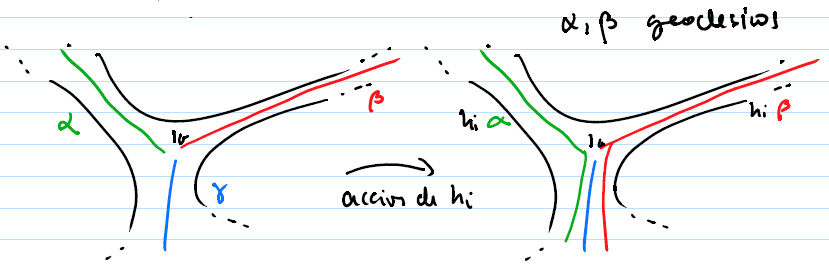
\includegraphics[scale=0.5]{dibu}
\end{figure}

Existe $R$ tal que $\{a_i\}_{i\geq R}$ y $\{b_i\}_{i\geq R}$ no pueden ser conectados por un 1-camino fuera de la bola $B(1_G,R)$. En particular, $d(a_i,b_i)>2R$. Como $\gamma$ es equivalente a $\alpha$ ni a $\beta$, para todo $c_l$ y para $i$ suficientemente grande existe $h_l\in H$ tal que $d(c_l,h_l)\leq k$ y tal que $h_l\alpha\sim \alpha$ y $h_l\beta\sim\beta$ y por tanto $h_l\alpha$ y $h_l\beta$ pasan por la bola $B(1_G,R)$. Entonces existe $i>2R$ y existe $h$ tal que $d(ha_i,hb_i)\leq 2R$.
\QED
\end{dem}

\begin{ej}[grupo con infinitos finales]
Sea $\F_2=\gene{a,b\mid}$ el grupo libre en 2 generadores.

\begin{figure}[h!]
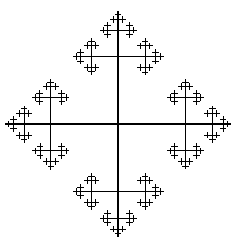
\includegraphics[scale=0.7]{cover}
\end{figure}
Obsérvese que de hecho la cantidad de finales es no numerables puesto que tiene la cardinalidad del conjunto de Cantor. 
\end{ej}

Terminamos la sección con un teorema.

\begin{teorema}
Las siguientes afirmaciones son equivalentes:
\begin{enumerate}
\item $G$ tiene un subgrupo cíclico infinito de índice finito.
\item $G\sim_{QI}\Z$.
\item $|Ends(G)|=2$.
\end{enumerate}
\end{teorema}
\begin{dem}
Solo falta $3\Rightarrow 1$. Fijamos un grafo de Cayley $\Gamma(G,X)$. Sean $\alpha$ y $\beta$ dos rayos geodésicos empezando en $v$ y tal que existe $R\geq 0$ tal que $\alpha$ y $\beta$ están contenidos componentes conexas distintas  de $\Gamma(G,X)-B(v,R)$.

\definecolor{qqqqff}{rgb}{0.,0.,1.}
\definecolor{ffqqqq}{rgb}{1.,0.,0.}
\begin{tikzpicture}[line cap=round,line join=round,>=triangle 45,x=1.0cm,y=1.0cm]
\clip(-5.,-0.5) rectangle (5,2.5);
\draw [line width=2.pt,domain=-8.88:14.12] plot(\x,{(--6.-0.*\x)/3.});
\draw [line width=2.pt,domain=-8.88:14.12] plot(\x,{(-0.-0.*\x)/3.});
\draw [line width=2.pt,dash pattern=on 5pt off 5pt] (0.,1.) circle (1.4cm);
\draw [line width=2.pt,color=ffqqqq,domain=0.0:14.120000000000001] plot(\x,{(--4.-0.*\x)/4.});
\draw [line width=2.pt,color=qqqqff,domain=-8.88:0.0] plot(\x,{(-3.58-0.02*\x)/-3.58});
\draw [line width=2.pt,dash pattern=on 5pt off 5pt] (0.,1.)-- (0.9797958971132712,2.);
\draw (0.02,2.08) node[anchor=north west] {$R$};
\begin{scriptsize}
\draw (0.,1.) circle (2.5pt);
\end{scriptsize}
\end{tikzpicture}

Existe $H\leq G$ con $[G:H]\leq 2$ tal que $H$ fija esos finales.

Existe $k$ tal que para todo $g\in G$ existe $h$ con $d(h,g)\leq k$. Tomamos $\CC=B(v,R)\cup$ componente de $\beta$. Sea $h\in H$ tal que $d(h,\beta(R+2k))\leq k$. Entonces $h\CC\subsetneq \CC$, luego $h^2\CC\subsetneq h\CC\subsetneq\CC$ etc. Con lo que el orden de $h$ es infinito. Falta ver que el índice de $\gene{h}$ es finito. 

Ahora, $\Gamma-(B(v,R)\cup hB(v,R))$ tiene dos componentes conexas infinitas y un número finito de componentes conexas finitas. Sea $D$ la unión de las componentes conexas finitas y $B(v,R)$. Entonces $\bigcup_{h\in\gene{h}} hD=\Gamma(G,X)$, luego $\bigcup_{d\in D}\gene{h}d=G$, por lo que $\gene{h}$ tiene índice finito en $G$.
\QED
\end{dem}

\section{Grupos finitamente presentados}
\subsection{Grupos libres}
\begin{defi}
Sea $X$ un conjunto, $L$ un grupo e $i:X\to L$ una función. Diremos que $(L,i)$ es \textbf{libre} en $X$ si para todo grupo $H$ y toda función $f:X\to H$ existe un único homomorfismo $\varphi:L\to H$ de modo que el siguiente diagrama conmuta
\[
\begin{tikzcd}
X\arrow[r, "f"]\arrow[d,"i"'] & H\\
L\arrow[ur, dashed, "\exists!\varphi"']
\end{tikzcd}
\]
\end{defi}

\begin{observacion}\label{4.2}
Sea $H=\gene{Y}$ un grupo. Sea $X$ un conjunto con $|X|>|Y|$ y $(L,i)$ el grupo libre en $X$. Como $|X|>|Y|$, podemos tomar $f:X\to H$ tal que $Y\subseteq f(X)$. Entonces existe $\varphi:L\to H$ homomorfismo sobreyectivo y tenemos que $H\cong L/\ker\varphi$.
\end{observacion}

\begin{defi}
Una presentación de $H$ es un grupo libre $(L,i)$ y un subgrupo $N\trianglelefteq L$ tal que $L/N\cong H$. 
\end{defi}

\begin{prop}\
\begin{enumerate}
\item Si $(L_1,i_1)$ y $(L_2,i_2)$ son libres en $X$ entonces existe $\varphi$ de modo que el siguiente diagrama conmuta
\[
\begin{tikzcd}
L_1\arrow[r, dashed,"\varphi"] & L_2\\
X\arrow[u, "i_1"]\arrow[ur, "i_2"]&
\end{tikzcd}
\]
\item Dado $(L,i)$ libre, $i$ es inyectiva. 
\item Si $(L_1,i_1)$ es libre en $X_1$ y $(L_2,i_2)$ es libre en $X_2$ entonces $L_1\cong L_2\Leftrightarrow |X|=|Y|$ (se puede suponer que $|X|,|Y|<\infty$).
\end{enumerate}
\end{prop}
\begin{dem}\
\begin{enumerate}
\item Basta considerar $H=L_2$ y $f=i_2$ en la definición de que $(L_1,i_1)$ sea libre en $X$. 
\item Basta considerar $H=\gene{X}$ y $f$ la inclusión natural de $X$ en $H$. Como $j$ es inyectivo, también lo es $\varphi\circ i$, de donde se deduce la inyectividad de $i$.
\item Supongamos que $L_1\cong L_2$. Tenemos entonces el siguiente diagrama
\[
\begin{tikzcd}
L_1\arrow[r, "\varphi", "\cong"'] & L_2\\
X\arrow[u, "i_1"] & Y\arrow[u, "i_2"]
\end{tikzcd}
\]
Con lo que $\varphi$ es en particular una biyección entre $i_1(X)$ e $i_2(Y)$, por lo que, gracias al primer apartado, necesariamente $|X|=|Y|$.

Supongamos ahora que $|X|=|Y|$, por lo que existe una biyección $g$ entre ambos conjuntos. Consideramos $f=i_2\circ g$, con lo que obtenemos el diagrama
\[
\begin{tikzcd}
L_1\arrow[r, dashed, "\varphi"] & L_2\\
X\arrow[u, "i_1"]\arrow[r,"g"] & Y\arrow[u, "i_2"]
\end{tikzcd}
\]
Como $f$ es inyectiva por composición, se deduce que $\varphi$ debe ser inyectiva, y por la observación \ref{4.2} tenemos las sobreyectividad.
\end{enumerate}
\QED
\end{dem}

\begin{teorema}
Dado un conjunto $X$, existe $(L,i)$ libre en $X$.
\end{teorema}
\begin{dem}
Sea $X^{-1}$ un conjunto en biyección con $X$ mediante $x\mapsto x^{-1}$. Por abuso de notación a la inversa también la denotamos $x\mapsto x^{-1}$. Sea $(X\cup X^{-1})^*$ el monoide de palabras en $X\cup X^{-1}$ con la yuxtaposición. Decimos que $w=y_1\cdots y_n\in (X\cup X^{-1})^*$ es \textbf{reducida} si $\forall\ 1\leq i\leq n-1$, $y_i\neq y_{i+1}^{-1}$. Si $w$ no es reducida, entonces $w=y_1\cdots y_iy_i^{-1}y_{i+2}\cdots y_n$, se ha obtenido a través de una \textbf{reducción elemental} y ponemos $w\to_r w'$. 

Dos palabras son equivalentes si están en la misma componente conexa del grafo con vértices $V\Gamma=(X\cup X^{-1})^*$ y aristas en las palabras relacionadas por reducciones elementales. 

\[
\begin{tikzcd}
zxx^{-}z\arrow[d] & zxx^{-1}y^{-1}y\arrow[l]\arrow[r] &zzy^{-1}y\arrow[lld]\\
zz 
\end{tikzcd}
\]

Entonces se tiene que $F(X)=(X\cup X^{-1})^*/\sim$ es un grupo libre en $X$ y existe una única palabra reducida en cada clase de equivalencia. La segunda afirmación es clara así que vamos a probar la primera. Consideramos $i:X\to F(X)$ la aplicación que envía cada elemento a su clase de equivalencia (de hecho son palabras reducidas). Sea $H$ un grupo y $f:X\to H$ una función. Definimos $\varphi:F(X)\to G$ a partir de las palabras reducidas como $x_{i_1})^{\varepsilon_1}\cdots x_{i_n}^{\varepsilon_n}\mapsto f(x_{i_1})^{\varepsilon_1}\cdots f(x_{i_n})^{\varepsilon_n}$. Cualquier homomorfismo de $F(X)\to G$ que haga que el diagrama conmute debe cumplir esa definición luego es único. Se puede ver con más detalle esta demostración en \url{https://www.math.unl.edu/~mbrittenham2/classwk/990s08/public/myasnikov.1.free.groups.pdf}

\QED
\end{dem}

Volvemos a las presentaciones. Dado $X$, el grupo libre en $X$ existe y es único salvo isomorfismo. Lo denotamos $\gene{X\mid\ }$. 

Dado $R\subseteq G$, $\gene{R^G}$ denota el subgrupo generado por todos los $G$-conjugados de $R$, es decir, $$\bigcap_{N\triangleleft G, N\subseteq R} N$$
Dado un conjunto $X$ y $R\subseteq\gene{X\mid\ }$ denotamos por $\gene{X\mid R}$ al grupo $\gene{X\mid\ }/\gene{R^{\gene{X\mid\ }}}$.

Por lo visto anteriormente, para todo grupo $G$ existe un conjunto $X$ y $R\subseteq\gene{X\mid\ }$ tal que $\gene{X\mid R}\cong G$.
\subsection{Transformaciones de Tietze}
\begin{teorema}[Von Dyck]
Sea $G=\gene{X\mid R}$, $H$ un grupo, $f:X\to H$ una función y $\varphi:\gene{X\mid\ }\to H$ el homomorfismo conocido. 
\begin{enumerate}
\item Si $\varphi(R)=\{	1_H\}$, entonces existe $\psi:G\to H$ tal que $\psi(x)=f(x)$.
\item Si además $f(X)$ genera $H$, entonces $\psi$ es sobreyectiva.
\end{enumerate}
\end{teorema}

Se conocen como \textbf{transformaciones de Tietze} los siguientes isomorfismos:
\begin{enumerate}
\item Si $s\in \gene{R^{\gene{X\mid\ }}}$, entonces $\gene{X\mid R}\cong\gene{X\mid R\cup\{s\}}$.
\item Si $y\notin X$ y $u\in\gene{X\mid\ }$, entonces $\gene{X\mid R}\cong \gene{X\cup \{y\}\mid R\cup \{yu\}}$.
\end{enumerate}

\begin{teorema}
Si $\gene{X\mid R}\cong\gene{X\mid R'}$ son presentaciones finitas, entonces se puede obtener una presentación de la otra mediante una sucesión finita de transformaciones de Tietze.
\end{teorema}

\subsection{El problema de la palabra}
En 1910 Max Dehn propuso tres problemas algorítmicos para grupos finitamente presentados que sentaron las bases de la teoría combinatoria de grupos. 
\begin{enumerate}
\item El problema dela palabra. Dado $G=\gene{X\mid R}$, ¿existe un algoritmo con entrada $w\in (X\cup X^{-1})^*$ y que decida si $w=_G1_G$ o no?
\item Problema de la conjugación. Dado $G=\gene{X\mid R}$, ¿existe un algoritmo con entrada $w,u\in (X\cup X^{-1})^*$ y que decida si existe $g\in G$ con $gw=_G ug$?
\item Problema del isomorfismo. ¿Existe algoritmo con entradas $\gene{X\mid R}, \gene{Y\mid S}$ finitas y decida si $\gene{X\mid R}\cong \gene{Y\mid S}$?
\end{enumerate}

En los años 1950 Boone y Novikov construyen un grupo finitamente presentado con problema de la palabra irresoluble. A su vez, Adyan y Rabin prueban que no existe un algoritmo que decida si una presentación finita es el grupo trivial. En la década de 1970 se encuentra un grupo con problema de la palabra resoluble pero problema de la conjugación irresoluble. 

Nos vamos a centrar en el problema de la palabra. Sea $G=\gene{X\mid R}$ finita y $w\in (X\cup X^{-1})^*$. Entonces $w=_G 1$ si y solo si $w\in \gene{R^{\gene{X\mid\ }}}$ si y solo si $w=\displaystyle\prod_{i=1}^M p_ir_i^{\varepsilon_i}p_i^{-1}$ en $\gene{X\mid\ }$, donde $r_i\in R, p_i\in\gene{X\mid\ }, \varepsilon_i=\pm 1$.

Si $w=_G 1$, definimos $Area(w)=\min\{M\mid w=\prod_{i=1}^M p_ir_i^{\varepsilon_i}p_i^{-1}\}$ y $Dehn_{\gene{X\mid R}}(n)=\max\{Area(w)\mid l(w)\leq n, w=1_G\}$.

\begin{ej}
$\gene{x,y\mid r=xyx^{-1}y^{-1}}$. Sea $w=y^4x^2y^{-1}x^{-2}y^{-3}$. Entonces
\[
w=(y^4ry^{-4})(y^{4}x^2rx^{-2}y^{-4})(y^{3}x^2rx^{-2}y^{-3})(y^3ry^{-3})
\]
PREGUNTAR A MENESES PORQUE NO ENTIENDO NADA
\end{ej}

\begin{ej}
$BS(1,2)=\gene{a,b\mid b^{-1}ab=a^2}\cong\left\langle\begin{pmatrix}
1 & 1\\
0 & 1
\end{pmatrix}, \begin{pmatrix}
2 & 0 \\
0 & 1
\end{pmatrix}\right\rangle\subseteq GL_2(\Q)$. DIBUJO Y FINAL DEL EJEMPLO
\end{ej}

Diremos que $f,g:\N\to\R_{\geq 0}$ son \textbf{equivalentes} (denotado $f\sim g$) si existe $A>0$ tal que
\begin{gather*}
f(n)\leq Ag(An+A)+An+A\\
g(n)\leq Af(An+A)+An+A
\end{gather*}
Esta equivalencia coincide con la de las funciones de crecimiento salvo que ahora las sub-lineales son equivalentes a las lineales. 

Se puede demostrar que $Dehn_{BS(1,2)}(n)\sim 2^n$.

\begin{lemma}
Dadas dos presentaciones finitas $\gene{X\mid R}\cong \gene{Y\mid S}$, sus funciones de Dehn son equivalentes.
\end{lemma}

La idea de la demostración de este lema es probarlo para transformaciones de Tietze. 

Sea $\gene{X\mid R}$ una presentación finita. Un \textbf{diagrama de Van Kampen}\footnote{\url{https://en.wikipedia.org/wiki/Van_Kampen_diagram}} con frontera $w$ es un grafo plano conexo con aristas orientadas con etiquetas en $X$, y en cada región interior las etiquetas son palabras de $R^{\pm 1}$ (empezando desde el vértice adecuado). Además existe un punto base en la frontera tal que la etiqueta de la frontera leída desde el punto base es $w$. 

\begin{teorema}
Dada $\gene{X\mid R}$ finita
\begin{enumerate}
\item si $w\in \gene{R^{\gene{X\mid }}}$ entonces existe diagrama de Van Kampen para $w$.
\item Si $D$ es un diagrama de Van Kampen para $w$, entonces $w=_G 1$.
\end{enumerate}
\end{teorema}

\begin{observacion}
Dado un diagrama de Van Kampen para $w$ podemos encontrar los $p_i$, los $r_i$ y $M$ tal que $w=\prod_{i=1}^M p_i r_i^{\varepsilon_i} p_i^{-1}$.

\begin{figure}[h!]
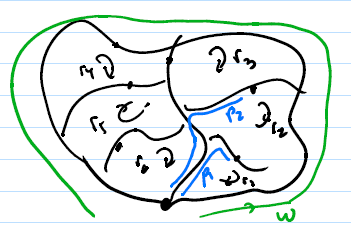
\includegraphics[scale=0.6]{palabra}
\end{figure}

En particular, $l(p_i)\leq l(\max_{r\in R} l(r))+l(w)$.
\end{observacion}

\begin{teorema}
Sean $G,H$ finitamente generados y quasi-isométricos. Si $G$ es finitamente presentable entonces $H$ es finitamente presentable y $Dehn_G\sim Dehn_H$.
\end{teorema}

\begin{coro}
Si $G$ es finitamente presentado y $H\leq G$ de índice finito, entonces $H$ tiene presentación finita.
\end{coro}

\begin{defi}
Una función $f:\N\to\N$ es \textbf{recursiva} si existe un algoritmo (máquina de Turing) con entrada $n$ y con salida $f(n)$. 
\end{defi}

\begin{teorema}
$Dehn_{\gene{X\mid R}}\leq f(n)$ con $f$ recursiva si y solo si $\gene{X\mid R}$ tiene problema de la palabra resoluble. 
\end{teorema}


\begin{coro}
Tener problema de la palabra resoluble es un invariante por quasi-isometría entre grupos finitamente presentables. 
\end{coro}

\section{Lenguas formales}

Hemos hablado repetidamente de palabras. Un conjunto $L\subseteq X^*$ se llama \textbf{lengua formal}. Las lenguas formales están clasificadas por la complejidad que tiene describirlas. Chomsky propuso la siguiente jerarquía:

\definecolor{qqqqff}{rgb}{0.,0.,1.}
\definecolor{ffqqff}{rgb}{1.,0.,1.}
\definecolor{ffqqqq}{rgb}{1.,0.,0.}
\begin{tikzpicture}[line cap=round,line join=round,>=triangle 45,x=1.0cm,y=1.0cm]
\clip(-2.1,-0.1) rectangle (18.1,4.1);
\draw[line width=2.pt,color=ffqqqq] (0.,0.) -- (0.,1.) -- (6.,1.) -- (6.,0.) -- cycle;
\draw[line width=2.pt,color=ffqqff] (0.,0.) -- (-1.,0.) -- (-1.,2.) -- (7.,2.) -- (7.,0.) -- cycle;
\draw[line width=2.pt,color=qqqqff] (-1.,0.) -- (-2.,0.) -- (-2.,3.) -- (8.,3.) -- (8.,0.) -- cycle;
\draw (0.1,0.75) node[anchor=north west] {Regular - Finite State Automata};
%\draw [line width=2.pt,color=ffqqqq] (0.,0.)-- (0.,1.);
%\draw [line width=2.pt,color=ffqqqq] (0.,1.)-- (4.,1.);
%\draw [line width=2.pt,color=ffqqqq] (4.,1.)-- (4.,0.);
%\draw [line width=2.pt,color=ffqqqq] (4.,0.)-- (0.,0.);
%\draw [line width=2.pt,color=ffqqff] (0.,0.)-- (-1.,0.);
%\draw [line width=2.pt,color=ffqqff] (-1.,0.)-- (-1.,2.);
%\draw [line width=2.pt,color=ffqqff] (-1.,2.)-- (5.,2.);
%\draw [line width=2.pt,color=ffqqff] (5.,2.)-- (5.,0.);
%\draw [line width=2.pt,color=ffqqff] (5.,0.)-- (0.,0.);
\draw (-0.2,1.7) node[anchor=north west] {Context-free - push-down automata};
%\draw [line width=2.pt,color=qqqqff] (-1.,0.)-- (-2.,0.);
%\draw [line width=2.pt,color=qqqqff] (-2.,0.)-- (-2.,3.);
%\draw [line width=2.pt,color=qqqqff] (-2.,3.)-- (6.,3.);
%\draw [line width=2.pt,color=qqqqff] (6.,3.)-- (6.,0.);
%\draw [line width=2.pt,color=qqqqff] (6.,0.)-- (-1.,0.);
\draw (-1.25,2.74) node[anchor=north west] {Recursivamente enumerable - Máquina de Turing};
\draw (1.08,3.72) node[anchor=north west] {Lengua - Máquina};
\end{tikzpicture}


\subsection{Autómatas finitos (Finite State Automata)}

Un autómata es una máquina que hace cálculos. En este caso nos interesan los autómatas más sencillos (los autómatas finitos o FSA) que en el fondo no son más que un grafo finito dirigido en el que las arista tienen etiquetas de un alfabeto $A$ y tenemos un vértice inicial $\square$ y vértices finales $\odot$.

\begin{ej}
$A=\{0,1\}$.

\begin{tikzpicture}[line cap=round,line join=round,>=triangle 45,x=1.0cm,y=1.0cm]
\clip(-4.055,-1.9993749999999952) rectangle (13.91375,2.7975);
\draw[line width=2.pt] (0.,0.) -- (0.,1.) -- (-1.,1.) -- (-1.,0.) -- cycle;
\draw [line width=2.pt] (0.,0.)-- (0.,1.);
\draw [line width=2.pt] (0.,1.)-- (-1.,1.);
\draw [line width=2.pt] (-1.,1.)-- (-1.,0.);
\draw [line width=2.pt] (-1.,0.)-- (0.,0.);
\draw [->,line width=2.pt] (0.,0.5) -- (2.02,0.52);
\draw [line width=2.pt] (2.66,0.54) circle (0.640312423743285cm);
\draw [->,line width=2.pt] (3.3003124237432853,0.54) -- (4.94,0.54);
\draw [line width=2.pt] (5.6,0.52) circle (0.6603029607687664cm);
\draw [line width=2.pt] (5.6,0.52) circle (0.32249030993194133cm);
\draw [shift={(5.84,1.5)},line width=2.pt]  plot[domain=-1.2019796152205329:3.7626746558478077,variable=\t]({1.*0.5068227168871041*cos(\t r)+0.*0.5068227168871041*sin(\t r)},{0.*0.5068227168871041*cos(\t r)+1.*0.5068227168871041*sin(\t r)});
\draw [shift={(6.34,-0.26)},line width=2.pt]  plot[domain=-3.4294755808554855:1.849130089903287,variable=\t]({1.*0.5478963864751486*cos(\t r)+0.*0.5478963864751486*sin(\t r)},{0.*0.5478963864751486*cos(\t r)+1.*0.5478963864751486*sin(\t r)});
\draw [->,line width=2.pt] (5.367236715213333,1.317341458150606) -- (5.456760176421417,1.164579206103622);
\draw [->,line width=2.pt] (6.405279235842623,0.28399363202185424) -- (6.1974544680222685,0.23884495622481466);
\draw (0.76,1.11) node[anchor=north west] {$0$};
\draw (3.6,1.235) node[anchor=north west] {$0$};
\draw (5.72625,2.5475) node[anchor=north west] {$1$};
\draw (6.8,0.4225) node[anchor=north west] {$0$};
\end{tikzpicture}

Asociado al autómata tenemos el conjunto $\mathcal{L}$ de las palabras que leemos empezando en $\square$ y acaban en $\odot$. En el ejemplo, $L$ está generado por la expresión regular $00\{0,1\}^*$.
\end{ej}

\begin{ej}
$A=\{a,b,a^{-1},b^{-1}\}$. 

\begin{tikzpicture}[line cap=round,line join=round,>=triangle 45,x=1.0cm,y=1.0cm]
\clip(-4.3,-4.) rectangle (18.7,4.);
\draw[line width=2.pt] (1.,0.) -- (1.,1.) -- (0.,1.) -- (0.,0.) -- cycle;
\draw [line width=2.pt] (1.,0.)-- (1.,1.);
\draw [line width=2.pt] (1.,1.)-- (0.,1.);
\draw [line width=2.pt] (0.,1.)-- (0.,0.);
\draw [line width=2.pt] (0.,0.)-- (1.,0.);
\draw [->,line width=2.pt] (0.48,1.) -- (0.5,2.);
\draw [->,line width=2.pt] (1.,0.52) -- (2.02,0.54);
\draw [->,line width=2.pt] (0.,0.52) -- (-1.02,0.48);
\draw [->,line width=2.pt] (0.52,0.) -- (0.52,-1.06);
\draw [line width=2.pt] (0.54,-1.58) circle (0.5203844732503075cm);
\draw [line width=2.pt] (0.52,2.58) circle (0.5803447251418764cm);
\draw [line width=2.pt] (2.6,0.54) circle (0.58cm);
\draw [line width=2.pt] (-1.58,0.5) circle (0.560357029044876cm);
\draw [line width=2.pt] (0.52,2.58) circle (0.3805259518088088cm);
\draw [line width=2.pt] (2.6,0.54) circle (0.36221540552549664cm);
\draw [line width=2.pt] (-1.58,0.5) circle (0.4019950248448356cm);
\draw [line width=2.pt] (0.54,-1.58) circle (0.360555127546399cm);
\draw [->,line width=2.pt] (-1.3062076678040349,0.9889148789213662) -- (0.,2.322318025465498);
\draw [->,line width=2.pt] (2.2552531845713926,1.0064221620504687) -- (0.9971549014733057,2.2496619912877116);
\draw [->,line width=2.pt] (-1.3270177871865296,0.) -- (0.03515290608413513,-1.7062117734789661);
\draw [->,line width=2.pt] (2.388339895114832,0.) -- (1.048833194192552,-1.6890356844698324);
\draw [shift={(3.3,1.12)},line width=2.pt]  plot[domain=-1.9508989222070579:3.4633432079864352,variable=\t]({1.*0.414509879115845*cos(\t r)+0.*0.414509879115845*sin(\t r)},{0.*0.414509879115845*cos(\t r)+1.*0.414509879115845*sin(\t r)});
\draw [shift={(1.22,3.34)},line width=2.pt]  plot[domain=-1.874571316370396:3.6272147468872618,variable=\t]({1.*0.5568886620589937*cos(\t r)+0.*0.5568886620589937*sin(\t r)},{0.*0.5568886620589937*cos(\t r)+1.*0.5568886620589937*sin(\t r)});
\draw [shift={(-2.58,0.84)},line width=2.pt]  plot[domain=-0.06271442235095126:5.521828293242994,variable=\t]({1.*0.5320441419076678*cos(\t r)+0.*0.5320441419076678*sin(\t r)},{0.*0.5320441419076678*cos(\t r)+1.*0.5320441419076678*sin(\t r)});
\draw [shift={(0.58,-2.44)},line width=2.pt]  plot[domain=-4.077787307888048:0.9761836803465909,variable=\t]({1.*0.509746478061798*cos(\t r)+0.*0.509746478061798*sin(\t r)},{0.*0.509746478061798*cos(\t r)+1.*0.509746478061798*sin(\t r)});
\draw [->,line width=2.pt] (1.7459795574366983,3.1570505887176705) -- (1.4073019261260458,2.815554606847072);
\draw [->,line width=2.pt] (3.7140407110208256,1.1002837756656747) -- (3.4853744534096496,0.7492510931807002);
\draw [->,line width=2.pt] (0.6753797379996441,-2.9407436244981318) -- (1.0494598126424535,-2.638617613041038);
\draw [->,line width=2.pt] (-3.077188725053523,1.0294052285918185) -- (-3.069025728784655,0.6304175448065761);
\draw (-3.6,0.6) node[anchor=north west] {$a^{-1}$};
\draw (3.98,1.4) node[anchor=north west] {$a$};
\draw (0.24,4.) node[anchor=north west] {$b$};
\draw (0.06,-2.78) node[anchor=north west] {$b^{-1}$};
\draw (1.96,-0.46) node[anchor=north west] {$b^{-1}$};
\draw (-1.2,-0.82) node[anchor=north west] {$b^{-1}$};
\draw (-0.96,2.12) node[anchor=north west] {$b$};
\draw (1.86,2.06) node[anchor=north west] {$b$};
\draw (0.72,1.78) node[anchor=north west] {$b$};
\draw (0.7,-0.1) node[anchor=north west] {$b^{-1}$};
\draw (1.44,0.48) node[anchor=north west] {$a$};
\draw (-0.8,0.36) node[anchor=north west] {$a^{-1}$};
\end{tikzpicture}

$\mathcal{L}=\{$ palabras reducidas en $A\}$.
\end{ej}

Dado un grupo $G$ y un conjunto de generadores $X$ finito, definimos la lengua $WP(G,X)=\{w\in (X\cup X^{-1})^*\mid w=_G 1\}$.

\begin{lemma}[Anisimov]
$WP(G,X)$ es regular si y solo si $G$ es finito.
\end{lemma}
\begin{proof}
Supongamos que $G$ es finito. Entonces $\Gamma(G,X)$ es un grafo finito con etiquetas de $X$. Una $w\in (X\cup X^{-1})^*$ satisface que $w=_G1$ si y solo si $w$ es la etiqueta de un camino en $\Gamma(G,X)$ que empieza y acaba en $1_G$, lo que nos da el autómata finito.

Supongamos que $G$ es infinito. Para todo $n\geq 1$ existe $w\in (X\cup X^{-1})^*$ tal que $l(w)\geq n$ y ninguna subpalabra de $w$ representa el elemento neutro. Supongamos que $WP(G,X)$ es regular y tomemos un autómata finito $M$ que reconoce $WP(G,X)$. Sea $n$ mayor que el número de estados de $M$. Entonces $w=uvu'$ con $M$ acabando en el mismo vértice al leer $u$ y $v$ (por el principio del palomar). Entonces $uu^{-1}=_G 1$ y $uvu^{-1}\neq_G 1$ (porque de lo contrario $v$ representaría al neutro), pero $M$ tiene que aceptar o rechazar ambas palabras. 
\end{proof}

\begin{observacion}
Que $WP(G,X)$ sea regular se preserva por quasi-isometrías. ¿Es un accidente o es un fenómeno general? ¿Que sea $WP(G,X)$ context-free es invariante por quasi-isometrías?
\end{observacion}

\subsection{Push-down Automata}

A nuestro FSA vamos a añadirle una memoria muy limitada. Tenemos un nuevo alfabeto $\Sigma$ y una pila. Podemos poner símbolos de $\Sigma$ de uno en uno en la pila y podemos quitarlo. Solo podemos leer el símbolo más alto en la pila y comprobar si la pila está vacía o no.

En cada turno, la máquina opera dependiendo del estado del vértice en que se encuentra, lo que haya en lo alto de la pila y lo que lea de entrada (en un turno puede no leer). La máquina se puede mover a otro estado (o no) y borrar o añadir un símbolo a la pila (o dejarla igual).

Formalmente, un push-down automata es una upla $M=(V,X,\Sigma, \delta, v_0, F)$, donde $V$ es un conjunto de estados, $X$ el alfabeto de entrada, $\Sigma$ el alfabeto de la pila, $v_0\in V$ un estado inicial, $F\subseteq V$ un conjunto de estados finales y $\delta:V\times (X\cup\{\varepsilon\})\times\Sigma^*\to V\times\Sigma^*$ es tal que $\delta(v,x,w)$ solo depende de la última letra de $w$. Esto es, $\delta(v,x,w)=(v',w')$, donde si $w=z_1\cdots z_n$ entonces $w'$ consiste en eliminar $z_n$ o en añadir un nuevo símbolo de $\Sigma$ a $w$ (o $w'=w$). 

El autómata empieza en $(v_0,\varepsilon)$. Escribimos $M\vdash_w^* (v,\xi)$ si es posible que $M$ llegue al estado $(v,\xi)$ después de leer $w$. $\mathcal{L}(M)=\{w\in X^*\mid M\vdash_w^* (v,\varepsilon), v\in F\}$ donde $\varepsilon$ es la palabra vacía. $L$ es contex-free si y solo si $L=\mathcal{L}(M)$ para algún push-down automata. 

\begin{ej}
Sea $X=\{x_1,\dots, x_n\}$. Vemos que $WP(\gene{X\mid\ }, X)$ es aceptado por un push-down automata $M$ cuyo único vértice final es el incial. Al leer un símbolo $x_i^{\varepsilon_i}\in (X\cup X^{-1})^*$, sino es el inverso de la última letra en la pila, la añadimos a la pila. En caso contrario eliminamos el último símbolo de la pila. 
\end{ej}

\begin{ej}
$L=\{a^mb^na^mb^n\mid m,n\in\N\}$ no es context-free. 
\end{ej}

\begin{lemma}
Sea $G$ un grupo y $X$ e $Y$ dos conjuntos de generadores finitos. Entonces $WP(G,X)$ es context-free si y solo si $WP(G,Y)$ lo es. 
\end{lemma}

Podemos entonces escribir $WP(G)$ sin ambigüedad para referirnos a $WP(G,X)$ si estamos hablando de ser context-free. 

\begin{lemma}
Si $G$ es un grupo finitamente generado y virtualmente libre, entonces $WP(G)$ es context-free. 
\end{lemma}
\begin{proof}
Sea $L\leq G$ libre de índice finito, de modo que $G=Lg_1\cup\cdots\cup Lg_n$. Sea $N=\bigcap_{i=1}^n g_i^{-1}Lg_i\trianglelefteq G$. Consideramos, para $a\in G$,
\begin{gather*}
a^{-1}g_i^{-1}Lg_ia=a^{-1}g_i^{-1}L^{-1}Lg_ia=(Lg_ia)^{-1}(Lg_ia)=(Lg_j)^{-1}(Lg_j)
\end{gather*}
Así que $\{Lg_1,\dots, Lg_n\}=\{Lg_1a,\dots, Lg_na\}$. Deducimos que $N$ tiene índice finito en $G$. En general, si $A$ y $B$ tienen índice finito, $G/A\times G/B$ es finito y $G$ actúa sobre él mediante $g(sA,tB)=(gsA,gtB)$. Se tiene además el estabilizador de la acción de $G$ es $A\cap B$, de donde se sigue que $[G:A\cap B]<\infty$\footnote{\url{https://en.wikipedia.org/wiki/Group_action\#Orbit-stabilizer_theorem_and_Burnside's_lemma}}.

Como $G$ es finitamente generado y $Ntrianglelefteq G$ es de índice finito, $N$ es finitamente generado. Así que sea $N=\gene{y_1,\dots, y_n\mid\ }$ y $Q/N=\gene{q_1,\dots, q_t\mid q_iq_j=q_{ij}}$ (la presentación dada por la tabla de multiplicar). Consideramos la aplicación $\pi: G\to Q$ dada por $g\mapsto gN$ y $d_i\in G$ tal que $\pi(d_i)=q_i$. Así que 
\begin{gather*}
d_iy_id_i^{-1}=u_{ij}\in N\\
d_id_j^{\varepsilon}=z_{i,\varepsilon,j}d_{ij}\in N
\end{gather*}
Entonces 
\[
\gene{y_1,\dots, y_n\mid d_iy_jd_i^{-1}=u_{ij}, d_id_j^{\varepsilon}=z_{i,\varepsilon,j}d_{ij}}
\]
es una presentación de $G$ ya que podemos usar las relaciones para transformar cualquier palabra a la forma $wd_i$ con $w\in (Y\cup Y^{-1})^*$ reducida. Esa palabra será la identidad si y solo si $\pi(d_i)=1$ y $w$ es vacía. 

Podemos usar esta presentación para codificar $M$. La pila se hace cargo de recordar la parte libre y el grafo finito tiene vértices $\{d_1,\dots, d_k\}$. Si estamos en $(d_i,w)$ y leemos $x\in (Y\cup Y^{-1})^*$ operamos en $w$ como antes, $d_ix=ud_i$. Si leemos $d_j$ operamos con $d_id_j^{\varepsilon}=z_{i,\varepsilon,j}d_{ij}$.
\end{proof}

Existe una caracterización (entre las referencias de Yago) de context-free con la que es fácil probar que $WP(G,X)$ es context-free si y solo si $\Gamma(G,X)$ es quasi-isométrico a un árbol. 

El siguiente teorema es esencialmente de Müller y Schupp. 

\begin{teorema}
Las siguientes afirmaciones son equivalentes.
\begin{enumerate}
\item $G$ es virtualmente libre.
\item $G$ es context-free.
\item $G$ es quasi-isométrico a un árbol.
\end{enumerate}
\end{teorema}

\section{Miscelánea. Para saber más}
Hemos visto que $Dehn_G\sim n$ es un invariante por quasi-isometrías. Los grupos con esta propiedad se llama \textbf{grupos hiperbólicos}.
\begin{teorema}
Sea $G$ un grupo y $X$ un conjunto finito de generadores. $Dehn_G\sim n\Leftrightarrow \exists\ \delta>0$ tal que en $\Gamma(G,X)$ todo triángulo geodésico es $\delta$-delgado. 
\end{teorema}\

\begin{figure}[h!]
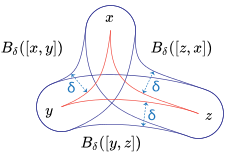
\includegraphics[scale=0.8]{delgado}
\caption{Triángulo $\delta$-delgado.}
\end{figure}

El concepto de $\delta$-hiperbólico es muy útil y en los últimos años se han llevado las ideas al límite (grupos relativamente hiperbólicos, grupos jerárquicamente hiperbólicos, grupos acíclicamente hiperbólicos...). Este concepto no depende del conjunto de generadores elegido.

Un teorema importante de Brady y Bridson afirma que el conjunto $\{\alpha\mid Dehn_G\sim n^{\alpha}\}$ es denso en $[2,\infty)$. Gromov probó que de hecho si $Dehn_G$ es sublineal, entonces debe ser lineal. 

En cuanto a los finales cabe destacar el siguiente teorema:
\begin{teorema}[Stallings]\footnote{\url{https://en.wikipedia.org/wiki/Stallings_theorem_about_ends_of_groups}}
$G$ tiene más de un final si y solo si $G=A*_C B$ o $G\cong HNN(A,C)$, en ambos casos con $C$ finito. 
\end{teorema}

El teorema se puede reformular como
\begin{teorema}
$G$ tiene más de un final si y solo si $G$ actúa en un árbol $T$ con una órbita de aristas y el estabilizador de una arista es finito.
\end{teorema}

Por último, comentamos el teorema de crecimiento polinómico de Gromov. 
\begin{teorema}
$\beta_G(n)\leq cn^d$ si y solo si $G$ es virtualmente nilpotente. 
\end{teorema}

\end{document}